\documentclass[twoside]{article}

\usepackage[preprint]{aistats2026}
\usepackage[utf8]{inputenc}
\usepackage[T1]{fontenc}
\usepackage[numbers,sort&compress]{natbib}
\usepackage{xcolor}
\definecolor{linkblue}{RGB}{0,90,160}

\usepackage{hyperref}
\hypersetup{
  colorlinks=true,
  citecolor=linkblue,
  linkcolor=linkblue,
  urlcolor=linkblue
}
\usepackage{booktabs}
\usepackage{adjustbox}
\usepackage{amsmath,amssymb,amsthm,amsfonts,mathtools}
\usepackage{graphicx}
\usepackage{subcaption}
\usepackage{float}
\captionsetup[subfigure]{font=footnotesize,justification=centering,singlelinecheck=false}
\usepackage{enumitem}
\usepackage{tikz}
\usetikzlibrary{arrows.meta,positioning,fit,backgrounds,shapes}
\usepackage{placeins}

\newtheorem{theorem}{Theorem}
\newtheorem{definition}{Definition}
\newtheorem{proposition}{Proposition}
\newtheorem{corollary}{Corollary}
\newtheorem{lemma}{Lemma}
\newtheorem{assumption}{Assumption}
\newtheorem{remark}{Remark}

\newcommand{\R}{\mathbb{R}}
\newcommand{\E}{\mathbb{E}}
\newcommand{\doo}{\mathrm{do}}
\newcommand{\An}{\mathrm{An}}
\newcommand{\QCBO}{\textsc{QCBO}}
\newcommand{\HQCBO}{\textsc{HQCBO}}
\newcommand{\QDCBO}{\textsc{QDCBO}}
\newcommand{\QMCBO}{\textsc{QMCBO}}
\newcommand{\CBO}{\textsc{CBO}}
\newcommand{\Gg}{\mathcal{G}}
\newcommand{\Gq}{\mathcal{G}^{\Pi}}
\newcommand{\ES}{\mathbf{ES}}
\newcommand{\ESpi}{\mathbf{ES}^{\Pi}}

\definecolor{okorange}{HTML}{E69F00}
\definecolor{okblue}{HTML}{56B4E9}
\definecolor{okpurple}{HTML}{CC79A7}
\tikzset{
  obsnode/.style={circle,draw=black!75,minimum size=6.5mm,inner sep=1pt,font=\small},
  mannode/.style={obsnode,fill=okorange!45},
  tgtnode/.style={obsnode,fill=okblue!45},
  clbox/.style={draw=black!55,dashed,rounded corners,inner sep=3.2mm},
  diredge/.style={->,>=Stealth,semithick,black!80},
  bicross/.style={<->,>=Stealth,okpurple,dashdotted,semithick},
  biintra/.style={bicross},
}

\begin{document}

\runningtitle{Coarsening Confers Robustness in Causal Bayesian Optimization}
\runningauthor{Anonymous}

\twocolumn[
\aistatstitle{Coarsening Confers Robustness: \\
Causal Bayesian Optimization under Graph Misspecification}
\aistatsauthor{Anonymous}
\aistatsaddress{Anonymous}
]

\begin{abstract}
Ignore the abstract for now

We need to write this, just writing here something so that the figure appears on the right side of the page 

for visual purposes only

right 

right

right

right

right

right

right
\end{abstract}

\section{Introduction}
\label{sec:intro}

Many scientific problems require choosing interventions in complex systems: which variables to act on, and at what values, to optimize a target under a limited experimental budget. Bayesian optimization (BO) fits a probabilistic surrogate to costly evaluations and selecting experiments sequentially. Standard BO, however, treats the system as a black box, i.e., it manipulates all inputs jointly without considering the causal structure enforced by the data-generating process (DGP). 

Causal Bayesian optimization (CBO)
\citep{agliettiCausalBayesianOptimization2020b} closes this gap by leveraging an assumed causal graph (specifically a directed acyclic graph (DAG)) to support the decision. Its assumed DAG determines which variables should be intervened on while observational data is used as prior information for interventional effects. This dependence on a correct graph is a fragile assumption since causal graphs are typically elicited from experts or estimated from finite data, and both sources can introduce errors. A misspecified DAG can not only slow learning but also exclude the best intervention from the search space. 

\begin{figure}[t]
  \centering
  % Motivating example (Fig. 1): three semantic subfigures.
\begin{subfigure}[t]{0.32\linewidth}
  \centering
  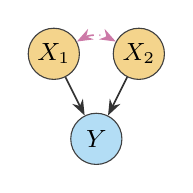
\begin{tikzpicture}[x=0.72cm,y=0.72cm]
    \node[mannode] (X1) at (0,1.15) {$X_1$};
    \node[mannode] (X2) at (1.5,1.15) {$X_2$};
    \node[tgtnode] (Y) at (0.75,-0.35) {$Y$};
    \draw[diredge] (X1) -- (Y);
    \draw[diredge] (X2) -- (Y);
    \draw[bicross] (X1) to[bend left=28] (X2);
  \end{tikzpicture}
  \caption{True graph}
  \label{fig:motivating-true}
\end{subfigure}\hfill
\begin{subfigure}[t]{0.32\linewidth}
  \centering
  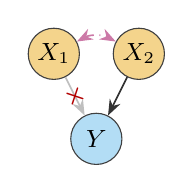
\begin{tikzpicture}[x=0.72cm,y=0.72cm]
    \node[mannode] (X1) at (0,1.15) {$X_1$};
    \node[mannode] (X2) at (1.5,1.15) {$X_2$};
    \node[tgtnode] (Y) at (0.75,-0.35) {$Y$};
    \draw[diredge,black!25] (X1) -- (Y)
      node[midway,sloped] {\textcolor{red!70!black}{\footnotesize$\boldsymbol{\times}$}};
    \draw[diredge] (X2) -- (Y);
    \draw[bicross] (X1) to[bend left=28] (X2);
  \end{tikzpicture}
  \caption{Assumed graph}
  \label{fig:motivating-assumed}
\end{subfigure}\hfill
\begin{subfigure}[t]{0.32\linewidth}
  \centering
  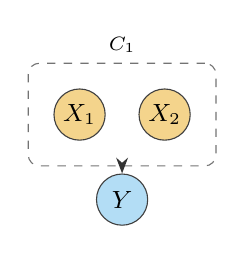
\begin{tikzpicture}[x=0.72cm,y=0.72cm]
    \node[mannode] (X1) at (0,1.15) {$X_1$};
    \node[mannode] (X2) at (1.5,1.15) {$X_2$};
    \node[tgtnode] (Y) at (0.75,-0.35) {$Y$};
    \begin{scope}[on background layer]
      \node[clbox,fit=(X1)(X2),label={[font=\scriptsize]above:$C_1$}] (C1) {};
    \end{scope}
    \draw[diredge] (C1.south) -- (Y);
  \end{tikzpicture}
  \caption{Common quotient}
  \label{fig:motivating-quotient}
\end{subfigure}

  \caption{The \textsc{ParallelParent} construction. Deleting
  $X_1\to Y$ changes the fine exploration set but not the quotient because the cluster edge $C_1\to Y$ remains through $X_2\to Y$. Orange nodes are manipulable, blue is the target, and the dash-dotted edge denotes latent
  confounding.}
  \label{fig:motivating}
\end{figure}

Figure~\ref{fig:motivating} illustrates a possible failure mode. The confounded parents $X_1$ and $X_2$ jointly determine $Y$, and the optimum requires setting both variables. If the assumed variable-level DAG (fine graph) omits $X_1\to Y$, CBO discards every intervention containing $X_1$. 

This observation motivates protecting the optimizer from a misspecified assumed DAG. We therefore change the resolution of the graph supplied to the optimizer. A partition $\Pi$ groups the variables into disjoint clusters of variables. The associated cluster causal graph (C-DAG) then expresses partial causal knowledge (relations between clusters are assumed while structure within them is left open). In the example of Figure~\ref{fig:motivating} (c), the two variables are represented by the cluster $C_1=\{X_1,X_2\}$, hence the edge $C_1\to Y$ survives through $X_2\to Y$ and the whole-cluster intervention remains available.

To this end, we introduce Quotient CBO (QCBO). QCBO receives a partition and its quotient graph (a C-DAG) as inputs and restricts interventions to unions of manipulable clusters. Such clusters may encode a known subsystem, a policy module, or another domain-defined unit whose coarse causal relationships are more reliable than its internal structure. The present work does not learn the partition or the quotient graph and assumes this is provided by the practitioner. Coarsening removes sensitivity to distinctions within clusters, but it can also hide useful fine-grained actions. Furthermore, in Figure~\ref{fig:motivating}, deleting both parent edges removes $C_1\to Y$ and changes the C-DAG itself. Such quotient-visible errors remain harmful; hence, a misspecified C-DAG hurts QCBO just as a misspecified DAG hurts CBO. 

Our contributions are threefold: 

\begin{enumerate}
    \item We formalize the \emph{quotient contract}: every graph-dependent component of the optimizer factors through the quotient. This implies that two runs supplied with different fine graphs having the same quotient select the same arms and intervention values.
    \item We characterize the price of restricting the action space to cluster unions, establish monotonicity under refinement, and give structural conditions for zero price. 
    \item We instantiate the contract for arm-based, dynamic, and model-based causal Bayesian optimizers and evaluate the predicted invariances and trade-offs. 
    
   
\end{enumerate} 
 Proofs, complete dataset graphs, and additional results are provided in the appendices.

\section{Problem setup and quotient construction}
\label{sec:setup}

\subsection{Causal Bayesian optimization}

Let
$\mathcal M=\langle\mathbf U,\mathbf V,F,P(\mathbf U)\rangle$ be a structural causal model (SCM), where \(\mathbf U\) and \(\mathbf V\) are the exogenous and endogenous variables, respectively; \(P({\mathbf U)}\) is the joint distribution of \(\mathbf U\); and \(F=\{f_V:V\in\mathbf V\}\) contains the structural assignments
\[
V := f_V\!\left(\operatorname{Pa}(V),\mathbf U_V\right),
\qquad V\in\mathbf V,
\] with \(\operatorname{Pa}(V)\subseteq\mathbf V\setminus\{V\}\) being the parents of $V$ (\(\operatorname{An}(V)\) for ancestors of $V$) and \(\mathbf U_V\subseteq\mathbf U\). Let \(Y\in\mathbf V\) be the target variable and let \(\mathbf X\subseteq\mathbf V\setminus\{Y\}\) be the set of manipulable variables \citep{pearlCausality2009}. The latent projection of \(\mathcal M\) onto \(\mathbf V\) is an acyclic directed mixed graph (ADMG) \(\mathcal G\), whose directed edges encode causal relations and whose bidirected edges encode latent confounding. Population expectations and interventional outcomes are always defined with respect to the data-generating SCM \(\mathcal M\). A hypothesis graph \(\widehat{\mathcal G}\) supplied to an optimizer can affect its decisions, but never the data-generating distribution.

An intervention arm is a nonempty set $A\subseteq\mathbf X$. Let $D(A)$ denote the intervention domain for the variables in $A$. For minimization, the population value of an arm is the setting of the arm that minimises the target in expectation:
\begin{equation}
  \mu^\star(A):=\min_{a\in D(A)}
  \E_{\mathcal M}\!\left[Y\mid\doo(A=a)\right].
  \label{eq:arm-value}
\end{equation}
CBO maintains a Gaussian process (GP) for each retained arm. CBO's exploration set ($\ES$) consists of the graph's minimal intervention sets (MIS) \citep{leeStructuralCausalBandits,agliettiCausalBayesianOptimization2020b}.
Writing ${\widehat{\mathcal G}}_{\bar A}$ for the graph obtained by deleting incoming edges to $A$, the MIS are
\begin{equation}
  \ES({\widehat{\mathcal G}})=\mathrm{MIS}({\widehat{\mathcal G}})
  :=\left\{A\subseteq\mathbf X:
  \substack{A\ne\emptyset,\\
  A\subseteq\An(Y)\text{ in }{\widehat{\mathcal G}}_{\bar A}}\right\}.
  \label{eq:mis}
\end{equation}
Equation~\eqref{eq:mis} filters candidate arms. For each nonempty $A\subseteq\mathbf X$, we form $\widehat{\mathcal G}_{\bar A}$ and retain $A$ if every member of $A$ remains an ancestor of $Y$.
For every retained arm $A$, CBO places a GP prior on the interventional response surface

\begin{equation}
  f_A(a):=\E_{\mathcal M}[Y\mid\doo(A=a)],
  \quad f_A\sim\mathcal{GP}(m_A^{\widehat{\mathcal G}},k_A)
  \label{eq:cbo-gp}
\end{equation}

for mean and covariance functions $m^\widehat{\mathcal G}_A$ and $k_A$. The GP prior mean incorporates observational information whenever the
interventional effect is identified under the supplied graph $\widehat{\mathcal G}$:
\begin{equation}
  m_A^{\widehat{\mathcal G}}(a)
  :=
  \widehat{\E}_{\widehat{\mathcal G}}\!\left[Y\mid\doo(A=a)\right].
  \label{eq:causal-prior}
\end{equation}
The identification procedure and the plug-in estimators used to evaluate Equation~\eqref{eq:causal-prior} are described in Appendix~\ref{app:estimators}. If the effect is not identified, we instead use the observational mean as an uninformative prior.

After collecting interventional data for arm $A$, let $\mu_{A,t}(a)$ and $\sigma_{A,t}(a)$ denote its GP posterior mean and standard deviation. Let $\mathcal D_0$ be the initial data. After $t$ sequential evaluations, let
\[
\mathcal D_t
:=
\mathcal D_0
\cup
\{(A_s,a_s,y_s)\}_{s=1}^{t},
\]
\[
y_t^{\mathrm{best}}
:=
\min\{y:(A,a,y)\in\mathcal D_t^{\mathrm{int}}\}.
\]
For minimization, the expected improvement over the
best observed outcome $y_t^{\mathrm{best}}$ is

\begin{equation}
  \operatorname{EI}_{A,t}(a)
  =
  \E\!\left[
    \bigl(y_t^{\mathrm{best}}-f_A(a)\bigr)_+
    \mid\mathcal D_t
  \right].
  \label{eq:ei}
\end{equation}
CBO selects
\begin{equation}
  (A_{t+1},a_{t+1})
  \in
  \arg\max_{\substack{A\in\ES({\widehat{\mathcal G}})\\a\in D(A)}}
  \frac{\operatorname{EI}_{A,t}(a)}{c(A,a)},
  \label{eq:cost-ei}
\end{equation}
where $c(A,a)$ is the intervention cost.

A common alternative is Gaussian Process Upper Confidence Bound (GP-UCB), with the corresponding minimization rule
given by GP-LCB (Lower):
\begin{equation}
  \operatorname{UCB/LCB}_{A,t}(a)
  =
  \mu_{A,t}(a)
  \pm
  \sqrt{\beta_t}\sigma_{A,t}(a).
  \label{eq:confidence-bounds}
\end{equation}
where $\beta_t>0$ controls exploration.

For a complete optimization run, let
\[
  \xi:=(\mathcal M,\mathcal D_0,\omega,\eta)
\]
collect the fixed true SCM $\mathcal M$, initial data $\mathcal D_0$, random stream $\omega$, and optimizer hyperparameters $\eta$. The true SCM is part of the environment rather than an input to the optimizer.

Thus an assumed graph ${\widehat{\mathcal G}}$ enters CBO through
\begin{equation}
 {\widehat{\mathcal G}}\longmapsto
 \left(\ES({\widehat{\mathcal G}}),\{m_A^{\widehat{\mathcal G}}\}_{A\in\ES({\widehat{\mathcal G}})}\right)
 \longmapsto \tau_{\mathcal A}({\widehat{\mathcal G}},\xi),
 \label{eq:trajectory-map}
\end{equation}
where $m_A^{\widehat{\mathcal G}}$ is the prior-mean function computed under ${\widehat{\mathcal G}}$ and $\tau_{\mathcal A}({\widehat{\mathcal G}},\xi)$ is the complete optimization trajectory: selected arms, intervention values, observations.


\subsection{Quotients and cluster-union interventions}

For a partition $\Pi$ of $\mathbf V \setminus Y $, let $\chi:\mathbf V\to\Pi$ map each variable to its cluster. The quotient $\Gg^\Pi$ has a directed edge $\chi(u)\to\chi(v)$ whenever $u\to v$ is present in $\Gg$ and $\chi(u)\ne\chi(v)$; bidirected edges are mapped analogously. The partition is \emph{valid} when the directed quotient is acyclic, and we write
\begin{equation}
  Q_\Pi(\Gg):=(\Pi,\Gg^\Pi).
  \label{eq:quotient}
\end{equation}

We assume that a cluster containing a manipulable variable contains only manipulable variables. Let
\[
  \Pi_M:=\{C\in\Pi:C\subseteq\mathbf X\}
\]
be the collection of manipulable clusters. QCBO may intervene on any
nonempty union of these clusters:
\begin{multline}
  \mathcal U(\Pi)
  :=
  \{
    A\subseteq\mathbf X:
    A\neq\emptyset \\
     \text{ and } A\text{ is a union of clusters in }\Pi_M \}. \\
  \label{eq:cluster-actions}
\end{multline}


QCBO applies the MIS rule to the quotient and expands each selected cluster arm to its constituent variables.
Let $\Pi_{\mathrm{fine}} := \{\{v\}:v\in\mathbf V\}$ denote the finest partition, in which every variable forms its own cluster. Its quotient is the original fine graph. The coarsest partition, by contrast, is the one-block partition $\{\mathbf V\}$. The best population value reachable under $\Pi$ and its loss relative to the full fine action space are
\begin{equation}
  V(\Pi):=\min_{A\in\mathcal U(\Pi)}\mu^\star(A),
  \qquad
  \Delta(\Pi):=V(\Pi)-V(\Pi_{\mathrm{fine}}).
  \label{eq:price}
\end{equation}
We call $\Delta(\Pi)$ the \emph{price of coarsening}. For minimization, it is nonnegative. It measures the loss caused by the restricted action space. For example, if $\Pi$ contains the manipulable cluster $\{X_1,X_2\}$, then the fine action family contains $\{X_1\}$, $\{X_2\}$, and $\{X_1,X_2\}$, whereas the coarse family contains only $\{X_1,X_2\}$.

For an incumbent intervention $\hat a_t$ (the intervention with the best observed value so far) after trial $t$, let $\mu(\hat a_t)$ be its expected outcome under the true SCM and define
\begin{equation}
  y^\star:=V(\Pi_{\mathrm{fine}}),\qquad
  r_t:=\mu(\hat a_t)-y^\star,\qquad
  R_T:=\sum_{t=1}^{T}r_t.
  \label{eq:regret}
\end{equation}

\section{Quotient causal optimizers}
\label{sec:methods}

Each quotient method replaces only the graph-dependent components of its base optimizer.

\subsection{Arm-based QCBO}

QCBO receives the partition \(\Pi\) and the supplied quotient \(Q_\Pi(\widehat{\Gg})\). For $S\subseteq\Pi_M$, let $U_\Pi(S):=\bigcup_{C\in S}C$. Its exploration set is
\begin{equation}
 \ESpi=\left\{U_\Pi(S):
 \emptyset\ne S\subseteq\Pi_M,\quad
 S\subseteq\An(Y)\text{ in }\widehat{\mathcal G}_{\bar S}\right\}.
 \label{eq:qcbo-arms}
\end{equation}
For each arm, a complete identification procedure determines whether the observational distribution identifies its prior mean. When it does, QCBO evaluates the returned functional with GP plug-in estimates of the required observational conditionals. The implementation supports a sound cascade of backdoor adjustment, frontdoor adjustment, and $g$-computation. Appendix~\ref{app:estimators} records the functionals and numerical implementation. The resulting two-tier prior is
\begin{equation}
  m_A(a)=
  \begin{cases}
    \widehat{\E}[Y\mid\doo(A=a)] & \text{if identified in }\widehat{\mathcal G},\\
    \bar Y_{\mathrm{obs}} & \text{otherwise.}
  \end{cases}
  \label{eq:two-tier-prior}
\end{equation}
Non-identifiable effects therefore receive an uninformative prior and are
learned from interventions.

\begin{proposition}[Identity recovery]
\label{prop:identity}
At $\Pi=\Pi_{\mathrm{fine}}$, the quotient graph equals the fine graph, the QCBO
exploration set equals $\mathrm{MIS}(\widehat{\Gg})$, and the prior construction
coincides arm-by-arm with CBO.
\end{proposition}

\subsection{Dynamic and model-based variants}

Quotient Dynamic CBO (QDCBO) replaces each time-slice graph and its transitions by their quotients and uses joint cluster mechanisms within each slice \citep{agliettiDynamicCausalBayesian2021a}. Quotient Model-Based CBO (QMCBO) replaces node mechanisms by joint conditional cluster mechanisms
\[
 P(\mathbf X_C\mid\mathbf X_{\mathrm{pa}(C)}),
\]
which are composed along the quotient graph
\citep{sussexMODELBASEDCAUSALBAYESIAN2023}. Joint rather than marginal
mechanisms are required to preserve dependence between variables within a
cluster.

\begin{corollary}[Portability of the quotient contract]
\label{cor:portability}
QDCBO satisfies Proposition~\ref{prop:contract} within each time slice, and QMCBO satisfies it for the composed model. At the finest partition, where every variable forms its own cluster, QDCBO and QMCBO reduce to DCBO and MCBO.
\end{corollary}

The substituted objects are summarized below. The remaining acquisition and update logic is inherited from the base method.

\begin{center}
\small
\adjustbox{max width=\linewidth}{%
\begin{tabular}{@{}ll@{}}
\toprule
Family & Quotient-level object \\
\midrule
CBO $\to$ QCBO & intervention arms and causal priors \\
DCBO $\to$ QDCBO & time-slice cluster mechanisms \\
MCBO $\to$ QMCBO & joint cluster mechanisms \\
\bottomrule
\end{tabular}
}
\end{center}

\section{Robustness and the price of coarsening}
\label{sec:theory}

\subsection{Quotient invariance}
\label{sec:invariance}

For an ADMG $\Gg$ and valid partition $\Pi$, define the protected class
\begin{equation}
E_\Pi(\mathcal G)
:=
\left\{
\widehat{\mathcal G}:
\begin{array}{l}
\widehat{\mathcal G}\text{ is an ADMG over }\mathbf V,\\
Q_\Pi(\widehat{\mathcal G})=Q_\Pi(\mathcal G)
\end{array}
\right\}.
\label{eq:protected-class}
\end{equation}

This class contains within-cluster edits and cross-cluster edits that leave every quotient edge represented. It excludes edits that add or remove a quotient edge.

Let $\mathcal D$ denote the initial data, $\eta$ the hyperparameters, and $\omega$ the optimizer's complete internal random stream (equivalently, its random seed together with all subsequent random draws). The quotient contract requires every graph-dependent operation to use a hypothesis graph only through $Q_\Pi$. We write $\mathcal A(\widehat{\mathcal G},\xi)$ for a run under the supplied graph $\widehat{\mathcal G}$ and $\tau_{\mathcal A}(\widehat{\mathcal G},\xi)$ for its trajectory. 



\begin{proposition}[Exact quotient invariance]
\label{prop:contract}
When two runs use the same true SCM, initial data, random stream, and
hyperparameters,
\[
  Q_\Pi(\widehat{\mathcal G})=Q_\Pi(\widehat{\mathcal G'})
  \quad\Longrightarrow\quad
  \tau_{\mathcal A}(\widehat{\mathcal G},\xi)
  =
  \tau_{\mathcal A}(\widehat{\mathcal G'}, \xi).
\]
\end{proposition}

The two runs make the same first decision; because the true SCM is fixed, they receive the same coupled observation; induction then gives identical subsequent decisions and observations. In Figure~\ref{fig:motivating}, deleting $X_1\to Y$ is protected because $X_2\to Y$ preserves the quotient edge, whereas deleting both parent edges removes $C_1\to Y$ and is not protected.

\subsection{Monotonicity under refinement}
\label{sec:price}

We write $\Pi'\preceq\Pi$ to mean that $\Pi'$ \emph{refines} $\Pi$: every cluster of $\Pi'$ is contained in a cluster of $\Pi$. Refinement enlarges the set of representable interventions.

\begin{proposition}[Monotonicity and price of coarsening]
\label{prop:price}
For valid $\Pi'\preceq\Pi$,
\[
 \mathcal U(\Pi)\subseteq\mathcal U(\Pi'),
 \qquad
 0\le\Delta(\Pi')\le\Delta(\Pi).
\]
Moreover,
\[
 \Delta(\Pi)=0
 \iff
 \arg\min_{A\in\mathcal U(\Pi_{\mathrm{fine}})}\mu^\star(A)
 \cap\mathcal U(\Pi)\ne\emptyset.
\]
\end{proposition}

Or,

\[
\Delta(\Pi)=0
\iff 
\]
\[\iff \exists A^\star\in\mathcal U(\Pi)
\text{ such that }
\mu^\star(A^\star)=V(\Pi_{\mathrm{fine}}).
\]


The result is purely about population reachability. Even when $\Delta(\Pi)=0$, a partition can change intervention dimension, cost, arm count, and finite-budget behavior.

\subsection{Sufficient conditions for lossless coarsening}
\label{sec:zero-price}

An arbitrary variable-level intervention does not need to be a union of clusters. 

Let $\chi(x)$ denote the unique cluster containing $x$. For $A\subseteq\mathbf X$, define its \emph{cluster completion}
\[
A^\Pi
:=
\bigcup_{x\in A}\chi(x)
=
  \bigcup\{C\in\Pi:C\cap A\neq\emptyset\}.
\]
Because every $x\in A$ belongs to $\chi(x)$, we have $A\subseteq A^\Pi$. Thus $A^\Pi$ is the unique smallest union of complete clusters containing $A$. Moving from the fine intervention $A$ to the admissible coarse intervention $A^\Pi$ therefore requires additionally intervening on
\[
  B:=A^\Pi\setminus A.
\]

Under the fine intervention $\doo(A=a)$, the variables in $B$ are not fixed: 
they follow their structural equations. Let $B(a)$ denote this natural response. Let $Y(a)$ denote the outcome under $\doo(A=a)$, and let $Y(a,b)$ denote the outcome under the joint intervention $\doo(A=a,B=b)$. The admissible values of $B$ compatible with $a$ are:
\[
  D_B(a):=\{b:(a,b)\in D(A^\Pi)\}
\]
We write $\operatorname{supp}(B(a))$ for the support of the distribution of $B(a)$, that is, the set of values that $B(a)$ can attain. Additionally Semi-Markovian SCMs allow latent confounding, represented by bidirected edges in the latent-projection ADMG, and strictly generalize Markovian SCMs, which exclude such confounding.

\begin{proposition}[Sufficient conditions for zero price]
\label{prop:free}
Assume a semi-Markovian SCM. If, for every $A\subseteq\mathbf X$ and
$a\in D(A)$,
\[
  \operatorname{supp}(B(a))\subseteq D_B(a)
\]
and
\[
  B(a)\perp Y(a,b)
  \qquad\text{for every }b\in D_B(a),
\]
then 
\[
V(\Pi)=V(\Pi_{\mathrm{fine}})
\qquad\text{and}\qquad
\Delta(\Pi)=0.
\]
\end{proposition}

The support condition ensures that every value naturally attained by the additional variables can also be selected by a whole-cluster intervention. The independence condition ensures that fixing these variables does not remove dependence that improves the target. Indeed, consistency and independence give
\[
  \E[Y(a)]
  =
  \int \E[Y(a,b)]\,\mathrm dP_{B(a)}(b)
  \ge
  \min_{b\in D_B(a)}\E[Y(a,b)].
\]

Thus every fine intervention can be matched or improved by at least one admissible whole-cluster intervention.

\begin{definition}[Full intervention support]
\label{def:full-support}
A partition $\Pi$ has full intervention support if, for every
$A\subseteq\mathbf X$ and $a\in D(A)$,
\[
\operatorname{supp}(B(a))\subseteq D_B(a).
\]
\end{definition}

\begin{definition}[Cluster-contained confounding]
\label{def:ccc}

Represent the semi-Markovian SCM by a nonparametric structural equation model with mutually independent exogenous variables and augmented graph $\Gg^{\mathrm{aug}}$.

%Here nonparametric means that the structural mechanisms are not restricted to be linear, Gaussian, or members of a specified finite-dimensional family. 
 
For $A\subseteq\mathbf X$ and $B=A^\Pi\setminus A$, let $\mathbf U_B(A)$ be the exogenous ancestors of $B$ after $\doo(A)$ and let $\mathbf U_Y(A)$ be the exogenous ancestors of $Y$ after $\doo(A^\Pi)$. The partition has cluster-contained confounding when $\mathbf U_B(A)\cap\mathbf U_Y(A)=\emptyset$ for every $A\subseteq\mathbf X$.
\end{definition}

\begin{corollary}[Graphical zero-price condition]
\label{cor:zero-price}
In a semi-Markovian SCM, full intervention support and cluster-contained confounding imply $V(\Pi)=V(\Pi_{\mathrm{fine}})$ and $\Delta(\Pi)=0$.
\end{corollary}

This condition is sufficient but not necessary. 

\subsection{Protected-class regret separation}
\label{sec:separation}

Fix a true SCM $\mathcal M$ with graph $\Gg$. Outcomes are generated by $\mathcal M$, while the optimizer receives a hypothesis graph $\widehat{\mathcal G}$. Let $R_T(\mathcal A,\widehat{\mathcal G})$ denote the regret of a run using $\widehat{\mathcal G}$ at fixed $\xi$. We denote worst-case regret over the protected class by ``wc'':
\[
 R_T^{\mathrm{wc}}(\mathcal A,\Pi,\Gg)
 :=\sup_{\widehat{\mathcal G}\in E_\Pi(\Gg)}R_T(\mathcal A,\widehat{\mathcal G}).
\]
For a cluster-union incumbent, adding and subtracting the best value available at resolution $\Pi$ gives
\begin{equation}
 \mu(\hat a_t)-y^\star
 =\underbrace{V(\Pi)-y^\star}_{\text{coarsening gap}}
 +\underbrace{\mu(\hat a_t)-V(\Pi)}_{\text{optimization error}}.
 \label{eq:regret-decomposition}
\end{equation}
The first term is irreducible for a fixed action space and vanishes only when $\Delta(\Pi)=0$. The second measures error relative to the best coarse action and can converge to zero.

\begin{theorem}[Protected-class regret separation]
\label{thm:separation}
The following statements hold.
\begin{enumerate}[label=(\roman*),leftmargin=1.6em,itemsep=2pt,topsep=2pt]
  \item For every $\beta>0$, there exist a semi-Markovian SCM, a valid partition with $\Delta(\Pi)=0$, and a hypothesis $\widehat{\mathcal G}\in E_\Pi(\Gg)$ obtained by deleting one directed edge, such that every optimizer whose initial and sequential interventions lie in $\mathrm{MIS}(\widehat{\mathcal G})$ and whose incumbent is selected among executed interventions satisfies
  \[
    r_t\ge\beta\quad\text{for every }t,
    \qquad R_T^{\mathrm{wc}}(\mathcal A,\Pi,\Gg)\ge\beta T.
  \]
  \item If an optimizer satisfies Proposition~\ref{prop:contract}, executes only cluster-union interventions, and selects its incumbent among executed actions, then its trajectory is identical for every $\widehat{\mathcal G}\in E_\Pi(\Gg)$ and
  \[
  \begin{aligned}
  R_T^{\mathrm{wc}}(\mathcal A,\Pi,\Gg)
  &=R_T(\mathcal A,\Gg)\\
  &=T\Delta(\Pi)
   +\sum_{t=1}^{T}\bigl(\mu(\hat a_t)-V(\Pi)\bigr).
  \end{aligned}
  \]
\end{enumerate}
\end{theorem}

Part (i) shows that a quotient-invisible edge error can force a fine-graph method to incur linear regret even when coarsening is lossless. The restrictions on both the initial design and incumbent selection are needed: otherwise an optimizer could evaluate or recommend an intervention excluded by $\mathrm{MIS}(H)$. Part (ii) decomposes quotient regret into the unavoidable structural price $T\Delta(\Pi)$ and the remaining optimization error within the quotient action space.

\subsection{Adaptive refinement}
\label{sec:refinement}

\begin{proposition}[Linear regret floor]
\label{prop:floor}
For a fixed partition,
\[
 r_t\ge\Delta(\Pi)\quad\text{for every }t,
 \qquad R_T\ge T\Delta(\Pi).
\]
\end{proposition}

Hierarchical QCBO (HQCBO) begins from a coarse partition and follows a declared refinement hierarchy. When progress stalls, it splits clusters participating in the incumbent, rejects splits whose quotient is cyclic, retains observations for arms that remain available, and initializes only newly exposed arms.

\begin{definition}[Incumbent consistency]
\label{def:consistency}
The base optimizer is incumbent-consistent on the action space of a
partition $\Pi_J$ if continued optimization on that space satisfies
$\mu(\hat a_t)\to V(\Pi_J)$ almost surely.
\end{definition}

\begin{corollary}[Conditional refinement recovery]
\label{cor:recovery}
If the refinement schedule visits a valid partition $\Pi_J$ with
$\Delta(\Pi_J)=0$ and the base optimizer is incumbent-consistent on that
action space, then
\[
 r_t\longrightarrow0,
 \qquad R_T/T\longrightarrow0.
\]
\end{corollary}

The result is conditional on the declared hierarchy exposing a lossless partition and on the consistency of the base optimizer.

\begin{corollary}[Adaptive refinement invariance]
\label{cor:adaptive-invariance}
Let $\tau_{\mathcal H}$ denote the HQCBO trajectory under a declared
hierarchy $\mathcal H$. If the visited partitions are
$\Pi_0,\ldots,\Pi_J$, then
\[
 \left[\forall j,\ \Gg^{\Pi_j}=(\Gg')^{\Pi_j}\right]
 \Longrightarrow
 \tau_{\mathcal H}(\Gg)=\tau_{\mathcal H}(\Gg').
\]
\end{corollary}

\section{Experiments}
\label{sec:experiments}

\subsection{Evaluation design and datasets}
\label{sec:exp-design}

The evaluation separates four claims: robustness to exploration-set corruption, robustness to causal-prior corruption, the action-space price of coarsening, and portability of the quotient contract. Table~\ref{tab:experiment-map} summarizes this design. In every misspecification comparison, the true SCM, initial data, hyperparameters, and random stream are paired. Only the graph supplied to the optimizer changes.

The controlled suite uses three SCMs with closed-form population effects:
\textsc{ParallelParent}, \textsc{FrontDoor}, and \textsc{MediatedChain}.
Their fine graphs, partitions, and quotients appear in Appendix~\ref{app:dags}. Each SCM provides one shared observational dataset; the optimizer receives its first $n_{\mathrm{obs}}=100$ observations. All displayed disturbance variables in this suite are mutually independent standard Gaussians; shared latent variables induce the stated bidirected edges. Interventional outcomes, including the initial design, are evaluated using the exact population expectation $\E[Y\mid\doo(A=a)]$. We use $30$ paired seeds, three initial intervention points per arm, unit cost per intervened variable, and $T=50$ trials, increased to $60$ for
\textsc{MediatedChain}.

The portability suite follows each base method's released protocol. The CBO family contains ToyGraph, CompleteGraph (``Synthetic''), and SimplifiedCoralGraph, with $10$ seeds, $n_{\mathrm{obs}}=100$, ten initial points per arm, $40$ trials, and minimization. The Coral simulator is the linear-SEM benchmark introduced by \citet{agliettiCausalBayesianOptimization2020b}: its graph is based on a Bermuda reef ecosystem model and its mechanisms were fit to $50$ field observations. The DCBO family uses stationary, independent, and nonstationary synthetic temporal SEMs, with $20$ seeds, three time slices, ten trials per slice, and minimization. The MCBO family uses its ToyGraph and PSAGraph simulators with $20$ seeds, $T=100$, $\beta=10$, zero observation noise, and maximization. PSAGraph is the model-based harness's adaptation of the prostate-specific-antigen simulator used in the original CBO study.

We report four complementary quantities: the best-so-far population objective, cumulative incumbent regret for the controlled minimization experiments, paired trajectory deviation for testing exact invariance, and the final objective value with its standard error across seeds. The \emph{best-so-far population value} evaluates the incumbent in the true SCM. For the controlled minimization suite, \emph{cumulative incumbent regret} is Equation~\eqref{eq:regret}. \emph{Paired trajectory deviation} compares the selected arms, intervention values, and incumbents of coupled correct- and wrong-graph runs. For the portability suite we report the final value as mean $\pm$ standard error.

\begin{table*}[t]
\centering
\caption{Evaluation map. Arrow up for maximization and down for minimization objective give the objective direction.}
\label{tab:experiment-map}
\small
\adjustbox{max width=\textwidth}{%
\begin{tabular}{@{}lllllll@{}}
\toprule
Study & Data & Perturbation & Comparison & Objective & Primary metric & Purpose \\
\midrule
A & \textsc{ParallelParent} & delete $X_1\to Y$ & CBO versus QCBO & $\downarrow$ & regret; deviation & exploration-set robustness \\
B & \textsc{FrontDoor} & add $X_1\leftrightarrow M$ & CBO versus QCBO & $\downarrow$ & regret; deviation & prior robustness \\
C & \textsc{MediatedChain} & refine $\{X_1,X_2\}$ & CBO, QCBO, HQCBO & $\downarrow$ & value; regret & price and recovery \\
D & eight family tasks & quotient graph view & base versus quotient & $\downarrow/\uparrow$ & final objective value & portability \\
\bottomrule
\end{tabular}}
\end{table*}

\subsection{Exploration-set corruption}
\label{sec:exp-a}

The \textsc{ParallelParent} SCM is shown in Figure~\ref{fig:motivating} and
Appendix~\ref{app:dags}. Its structural equations are
\begin{equation}
 \begin{aligned}
 U&=0.4\varepsilon_0,\\ X_1&=U+0.3\varepsilon_1,\\
 X_2&=U+0.3\varepsilon_2,\\
 Y&=(X_1-2)^2+(X_2+2)^2
  +0.1\varepsilon_Y.
 \end{aligned}
 \label{eq:parallel-parent-scm}
\end{equation}
Under the correct graph, the fine MIS are
$\{X_1\}$, $\{X_2\}$, and $\{X_1,X_2\}$, and the joint arm attains
$y^\star=0$ at $(2,-2)$. Deleting $X_1\to Y$ from the hypothesis graph removes every arm containing $X_1$ and leaves only $\{X_2\}$. Its exact population optimum is $4.25$, so no amount of optimization under the wrong fine graph can close this gap.

After $50$ trials, correct-graph CBO reaches $0.0016\pm0.0002$, whereas misspecified CBO ends at $4.2500\pm0.0000$ (mean $\pm$ standard error). Their cumulative incumbent regrets are $4.21\pm0.37$ and $216.23\pm1.12$, respectively. The latter value is close to the structural lower bound $4.25T=212.5$; the excess is finite-budget optimization error within the misspecified action space.

For $\Pi=\{\{X_1,X_2\},\{Y\}\}$, the same deletion is invisible because $X_2\to Y$ preserves the quotient edge. The paired QCBO runs select the same arms and intervention values at every trial, and their incumbent trajectories have zero deviation. Figure~\ref{fig:minimal-misspec}(a) therefore separates a permanent fine-graph arm exclusion from exact quotient invariance. A quotient-visible $X_1\leftrightarrow Y$ perturbation serves as the negative control and changes the QCBO trajectory, with maximum paired incumbent deviation $21.45$.

\subsection{Prior corruption without arm loss}
\label{sec:exp-b}

The \textsc{FrontDoor} graph in Appendix~\ref{app:dags} contains
$X_1\to M\to Y$ and latent $X_1\leftrightarrow Y$. Its SCM is
\begin{equation}
 \begin{aligned}
 U&=0.4\varepsilon_0,\\ X_1&=U+0.3\varepsilon_1,\\
 M&=2X_1+0.2\varepsilon_M,\\
 Y&=2\!\left[1-\exp\!\left\{-\frac{(M-1)^2}{2(0.3)^2}\right\}\right]+U+0.1\varepsilon_Y.
 \end{aligned}
 \label{eq:frontdoor-scm}
\end{equation}
Its population objective is minimized by $\doo(M=1)$. Under the correct graph, $\doo(M)$ is identified by adjustment for $X_1$ and $\doo(X_1)$ by the frontdoor criterion. Adding a spurious $X_1\leftrightarrow M$ leaves the fine MIS unchanged but makes both prior means non-identifiable. This design therefore changes the prior while holding the available arms fixed.

Fine CBO loses its observational head start and accumulates additional regret while searching for the narrow optimum, but it can recover from interventional observations because the optimal arm remains available. The paired increase in cumulative regret is $5.91\pm1.04$ at $T=50$; the final values are $0.0003\pm0.0003$ under the correct graph and $0.0035\pm0.0022$ under the corrupted graph. This is a transient finite-budget effect rather than an action-space exclusion like in \ref{sec:exp-a}. The perturbation is internal to $\{X_1,M\}$ and disappears in the quotient, so the paired QCBO decisions and incumbent trajectories are identical. The right panel of Figure~\ref{fig:minimal-misspec} contrasts this transient fine-graph effect with exact quotient invariance.

\begin{figure}[t]
  \centering
  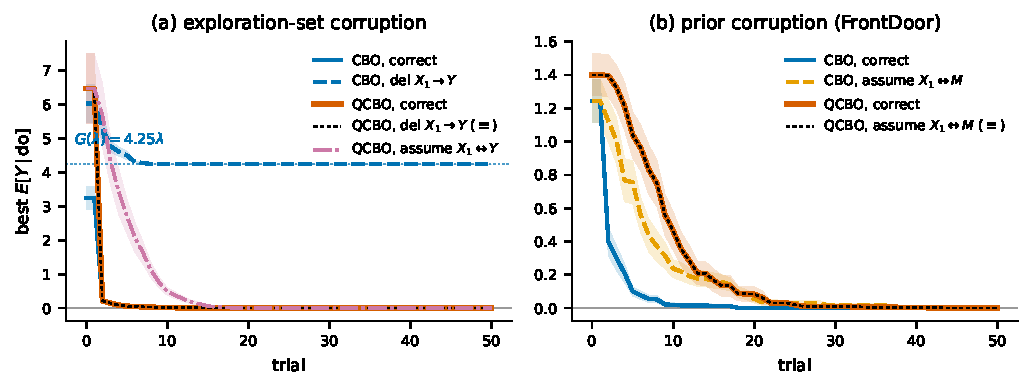
\includegraphics[width=0.90\linewidth]{figures/minimal_misspec}
  \caption{Correct and misspecified trajectories, mean $\pm$ standard error over $30$ seeds. Top: deleting $X_1\to Y$ removes the optimal fine arm, whereas QCBO is unchanged because the edit is invisible in the quotient. Bottom: corruption of an identified prior slows fine CBO, whereas QCBO remains exactly invariant.}
  \label{fig:minimal-misspec}
\end{figure}

\subsection{Action-space price and refinement}
\label{sec:exp-c}

The \textsc{MediatedChain}, in Appendix~\ref{app:dags}, graph has $X_1\to X_2\to Y$, with
\[
  X_2=2X_1+\varepsilon_2,
  \qquad
  Y=(X_2-4)^2+\varepsilon_Y.
\]
Fine CBO can execute $\doo(X_1=2)$ without intervening on $X_2$. The edge
$X_1\to X_2$ therefore remains active, giving
\[
  X_2=4+\varepsilon_2
  \quad\text{and}\quad
  \E[Y\mid\doo(X_1=2)]
  =
  \operatorname{Var}(\varepsilon_2)
  =
  0.04.
\]

Fixed QCBO cannot execute $\doo(X_1)$ alone because $X_1$ and $X_2$ belong
to the same manipulable cluster. Its only arm intervenes jointly:
\[
  \doo(X_1=x_1,X_2=x_2).
\]
Intervening on $X_2$ removes the edge $X_1\to X_2$, so $x_1$ no longer
affects the target. Since the intervention domain restricts
$x_2\in[-2,2]$, the best permitted value is
\[
  \min_{x_2\in[-2,2]}(x_2-4)^2=4.
\]
Hence
\[
  V(\Pi)=4,
  \qquad
  y^\star=0.04,
  \qquad
  \Delta(\Pi)=3.96.
\]

Consequently, every fixed-QCBO incumbent has instantaneous regret at least $3.96$, and Proposition~\ref{prop:floor} gives the permanent lower bound $R_T\ge3.96T$. Fine CBO does not incur this floor because its MIS retains $\{X_1\}$. HQCBO removes it only after the declared hierarchy splits $\{X_1,X_2\}$ and exposes the singleton arm. Figure~\ref{fig:minimal-refine} shows the resulting best-value and cumulative-regret trajectories. CBO, fixed QCBO, and HQCBO finish at $0.0400\pm0.0000$, $4.0000\pm0.0000$, and $0.0400\pm0.0000$, with cumulative regrets $5.46\pm1.61$, $243.23\pm0.90$, and $36.97\pm1.18$, respectively. HQCBO refines at trial $7.4\pm0.1$; all $30$ declared splits are accepted. The fixed-QCBO result exceeds the theoretical floor $60\times3.96=237.6$ only by its within-space optimization error. The experiment demonstrates recovery for this declared split; it does not imply that the plateau rule always selects a useful refinement.

\begin{figure}[t]
  \centering
  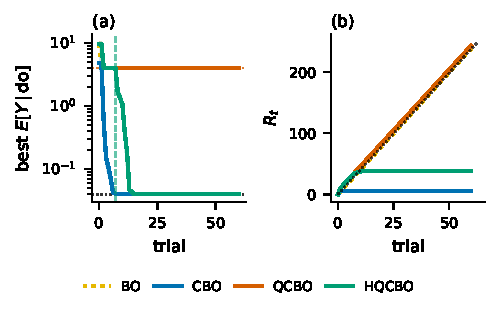
\includegraphics[width=0.90\linewidth]{figures/minimal_refine}
  \caption{Best-so-far population objective on
  \textsc{MediatedChain}, mean $\pm$ standard error over $30$ seeds.
  Fixed QCBO cannot execute $\doo(X_1)$; refinement exposes this arm.}
  \label{fig:minimal-refine}
\end{figure}

\subsection{Portability across optimizer families}
\label{sec:exp-d}

\begin{figure*}[t]
  \centering
  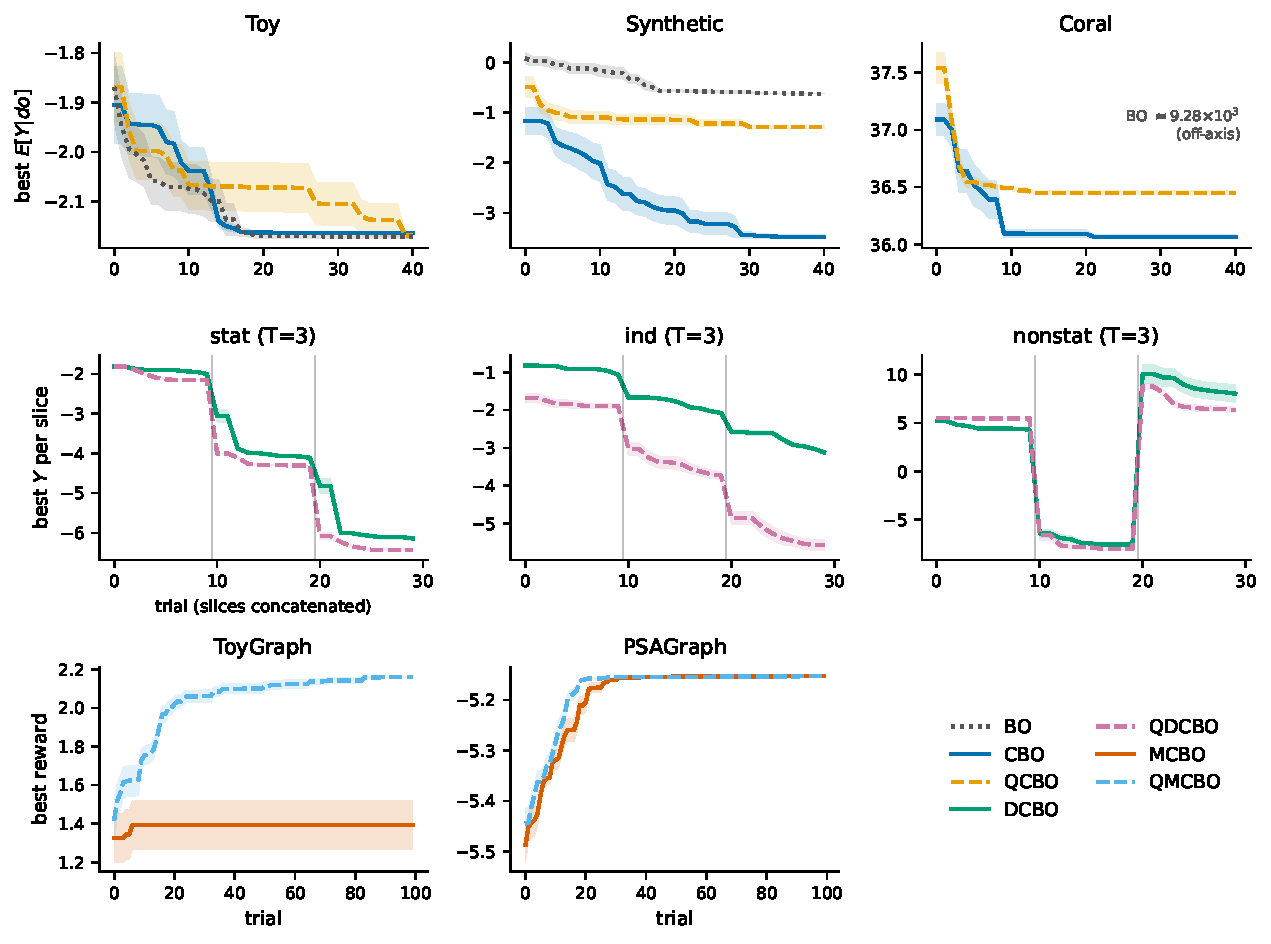
\includegraphics[width=\linewidth]{figures/family_suite}
  \captionsetup{width=\linewidth}
  \caption{Quotient methods and their corresponding base methods under the
  released family protocols, reported as mean $\pm$ standard error.
  Top: CBO minimization. Middle: dynamic minimization over three time
  slices. Bottom: MCBO maximization.} \colorbox{red}{MCBO HAS A PROBLEM I NEED TO FIX}
  \label{fig:family-suite}
\end{figure*}

Figure~\ref{fig:family-suite} compares each quotient construction with its base optimizer on the eight tasks described above; all corresponding DAGs and C-DAGs are in Appendix~\ref{app:dags}. The structural prediction is exact: QDCBO is invariant in all $60$ paired dynamic runs and QMCBO in all $40$ paired model-based runs, whereas their base methods change under the same graph-view perturbations. This confirms that the quotient contract is independent of the family-specific acquisition and surrogate construction.

Table~\ref{tab:family-finals} gives the final population value and paired quotient disadvantage for each task. For $\downarrow$ rows the paired difference is quotient minus base; for $\uparrow$ rows it is base minus quotient. Positive values therefore always mean that the quotient ended worse. 


\begin{table}[t]
  \centering
  \caption{Final objective value, reported as mean $\pm$ standard error
  across seeds. The arrows indicate the optimization direction:
  $\downarrow$ denotes minimization and $\uparrow$ maximization.}
  \label{tab:family-finals}
  \small
  \setlength{\tabcolsep}{5pt}
  \begin{tabular}{@{}lcc@{}}
    \toprule
    \textbf{Task} & \textbf{Base final} & \textbf{Quotient final} \\
    \midrule

    \multicolumn{3}{@{}l}{%
      \emph{\CBO{} vs.\ \QCBO{} ($n=10$ seeds)}} \\
    Toy $\downarrow$
      & $-2.16 \pm 0.00$ & $-2.13 \pm 0.03$ \\
    Synthetic $\downarrow$
      & $-3.14 \pm 0.19$ & $-1.25 \pm 0.07$ \\
    Coral $\downarrow$
      & $36.08 \pm 0.02$ & $36.42 \pm 0.01$ \\

    \addlinespace[3pt]
    \multicolumn{3}{@{}l}{%
      \emph{DCBO vs.\ \QDCBO{} ($3$ time slices; $n=20$ seeds)}} \\
    Stationary $\downarrow$
      & $-6.14 \pm 0.05$ & $-6.43 \pm 0.02$ \\
    Independent $\downarrow$
      & $-3.12 \pm 0.06$ & $-5.57 \pm 0.15$ \\
    Nonstationary $\downarrow$
      & $8.03 \pm 0.90$ & $6.33 \pm 0.29$ \\

    \addlinespace[3pt]
    \multicolumn{3}{@{}l}{%
      \emph{MCBO vs.\ \QMCBO{} ($n=20$ seeds)}} \\
    ToyGraph $\uparrow$
      & $1.39 \pm 0.13$ & $2.16 \pm 0.00$ \\
    PSAGraph $\uparrow$
      & $-5.15 \pm 0.00$ & $-5.15 \pm 0.00$ \\
    \bottomrule
  \end{tabular}
\end{table}

\clearpage

\section{Related work}
\label{sec:related}

Graph-agnostic and causal entropy optimization methods learn over candidate graphs online \citep{mukherjeeGraphAgnosticCausal2024,branchiniCausalEntropyOptimization2023}, while causal-bandit guarantees price learning an unknown graph within the horizon \citep{luCausalBanditsUnknown2021}. Our setting instead studies commitment to a fixed coarse input. These approaches are complementary: a graph learner could operate over, or trigger refinement of, a quotient.

The construction builds on cluster-DAG identification \citep{CausalEffectIdentification} and is related to causal abstraction and macro-level structure learning \citep{beckersAbstractingCausalModels2019,madaleno2026a}. We coarsen manipulable inputs and explicitly characterize the actions removed by that choice.

\section{Limitations}
\label{sec:limitations}

Exact invariance requires the correct quotient; quotient-visible errors and incorrect partitions remain harmful. The zero-price condition is sufficient and structural, and its cross-world consequence is not directly testable from single-world data. Refinement is heuristic, with recovery conditional on visiting a lossless partition and on consistency of the base optimizer. Different partitions also induce different arm counts, initialization costs, and intervention costs. Finally, QMCBO inherits the causal-sufficiency
assumption of its model-based factorization.

\section{Conclusion}
\label{sec:conclusion}

Coarsening makes precisely those graph distinctions that disappear in the quotient irrelevant to optimization. Within the resulting protected class, the complete trajectory is invariant. The price is the optimal value of fine interventions excluded by the partition, which is monotone under refinement and zero under the stated structural conditions. Theoretical and empirical results show that using quotients can prevent catastrophic graph errors, while hierarchical refinement provides a conditional route back to the fine action space.

\bibliographystyle{abbrvnat}
\bibliography{qcbo_aistats}

\appendix
\onecolumn
\raggedbottom

\section{Proofs and additional technical results}
\label{app:proofs}

\subsection{Minimal intervention sets and quotient values}
\begin{lemma}[MIS reduction]
\label{lem:mis-reduction}
Let $\mathcal G$ be an ADMG with manipulable variables $\mathbf X$
and target $Y$. For any $A\subseteq\mathbf X$, let
\[
  A'
  :=
  A\cap\An_{\mathcal G_{\bar A}}(Y),
\]
where $\mathcal G_{\bar A}$ is obtained by deleting all directed edges
entering vertices in $A$. Then:
\begin{enumerate}[label=(\roman*)]
  \item for every $a\in D(A)$,
  \[
    P\!\left(Y\mid\doo(A=a)\right)
    =
    P\!\left(Y\mid
      \doo\!\left(A'=a|_{A'}\right)\right);
  \]
  \item if $A'\ne\varnothing$, then
  $A'\in\operatorname{MIS}(\mathcal G)$;
  \item consequently, optimizing over
  $\{\varnothing\}\cup\operatorname{MIS}(\mathcal G)$ attains the same
  population optimum as optimizing over all subsets of $\mathbf X$.
\end{enumerate}
\end{lemma}


\begin{proof}
Set $R:=A\setminus A'$. We first show that, while $A'$ remains intervened on, no variable in $R$ can causally affect $Y$. Suppose for contradiction that some $r\in R$ has a directed path to $Y$ in $\mathcal G_{\bar A'}$. Such a path cannot enter a vertex of $A'$, because all directed edges entering $A'$ have been deleted. Let $r^\star$ be the last vertex of $R$ appearing on this path. The subpath from $r^\star$ to $Y$ contains no further vertex of $A$ and is therefore also present in $\mathcal G_{\bar A}$. Hence $r^\star\in\An_{\mathcal G_{\bar A}}(Y)$, contradicting $r^\star\in R=A\setminus A'$.

Thus, under $\doo(A'=a|_{A'})$, the variables in $R$ are not ancestors of $Y$. Replacing their natural structural mechanisms by the constants specified in $a|_R$ therefore leaves the distribution of $Y$ unchanged. This proves
\[
  P\!\left(Y\mid\doo(A=a)\right)
  =
  P\!\left(Y\mid
    \doo\!\left(A'=a|_{A'}\right)\right).
\]

It remains to show that a nonempty $A'$ is a minimal intervention set. For every $v\in A'$, there is a directed path from $v$ to $Y$ in $\mathcal G_{\bar A}$. After leaving $v$, this path cannot enter another vertex of $A$, since all directed edges entering $A$ have been deleted.
The same path is consequently present in $\mathcal G_{\bar A'}$, and
$v\in\An_{\mathcal G_{\bar A'}}(Y)$. Therefore
\[
  A'\subseteq\An_{\mathcal G_{\bar A'}}(Y),
\]
so $A'\in\operatorname{MIS}(\mathcal G)$ whenever $A'\ne\varnothing$.

Applying the first two statements to every $A\subseteq\mathbf X$ shows that each intervention is equivalent either to a minimal intervention set or, when $A'=\varnothing$, to the null intervention. Restricting the search to $\{\varnothing\}\cup\operatorname{MIS}(\mathcal G)$ therefore preserves the population optimum.
\end{proof}

Consequently, the best value over the quotient MIS expanded to fine variables equals $V(\Pi)$ in Equation~\eqref{eq:price}.

\colorbox{red}{I HAVE AN EXAMPLE WHERE THIS IS MAYBE EASIER TO UNDERSTAND, SHOULD WE ADD IT? OR UNECESSARY?}

\subsection{Proofs of the main structural results}

\begin{proof}[Proof of Proposition~\ref{prop:contract}]
Write the run as decisions $d_1,d_2,\ldots$ and datasets
$\mathcal D_0,\mathcal D_1,\ldots$, with
\[
d_t=f_t\!\left(Q_\Pi(\widehat{\mathcal G}),\mathcal D_{t-1},\omega_t,\eta\right).
\] 
Equal quotients, initial data, random streams, and hyperparameters imply equal first decisions. The fixed true SCM produces the same coupled observation, so the updated datasets also agree. Induction gives equality of every decision, observation, incumbent, and stopping event.
\end{proof}

\begin{proof}[Proof of Proposition~\ref{prop:price}]
Every union of clusters in $\Pi$ is a union of clusters in a refinement $\Pi'$, and every such union is available at the singleton partition. The three population minima are therefore taken over nested action families: $V(\Pi_{\mathrm{fine}})\le V(\Pi')\le V(\Pi)$. Equality between the first and last terms holds exactly when a global fine optimum belongs to $\mathcal U(\Pi)$.
\end{proof}

\begin{proof}[Proof of Proposition~\ref{prop:free}]
Fix $A$ and $a$. Consistency and cross-world independence give
\[
\begin{aligned}
 \E[Y_a]
 &=\int \E[Y_{a,b}\mid B(a)=b],dP(B(a)=b)\\
 &=\int \E[Y_{a,b}],dP(B(a)=b)\\
 &\ge \inf_{b\in D_B(a)}\E[Y_{a,b}],
\end{aligned}
\]
where support inclusion justifies the final inequality. Thus the whole cluster closure can match or improve every fine intervention: $\mu^\star(A^\Pi)\le\mu^\star(A)$. Taking minima and using $\mathcal U(\Pi)\subseteq\mathcal U(\Pi_{\mathrm{fine}})$ gives equality.
\end{proof}

\begin{lemma}[Cluster containment implies cross-world independence]
\label{lem:ccc} 
Under the model in Definition~\ref{def:ccc}, cluster-contained confounding implies $B(a)\perp Y_{a,b}$ for every $A$, $a$, and $b\in D_B(a)$.
\end{lemma}

\begin{proof}
Under $\doo(A=a)$, recursive substitution in the structural equations gives
\[
  B_a=f_B\bigl(\mathbf U_B(A);a\bigr),
\]
where $\mathbf U_B(A)$ contains the exogenous variables that remain
ancestors of $B$. Under
$\doo(A^\Pi=(a,b))$, the target can similarly be written
as
\[
  Y_{a,b}=f_Y\bigl(\mathbf U_Y(A);a,b\bigr).
\]
Cluster-contained confounding requires
$\mathbf U_B(A)\cap\mathbf U_Y(A)=\emptyset$. Because the exogenous variables of the nonparametric SCM are mutually independent, functions of these two disjoint sets are independent. Hence $B_a\perp Y_{a,b}$.
\end{proof}

\begin{proof}[Proof of Theorem~\ref{thm:separation}]
For part (i), use \textsc{ParallelParent} with manipulable variables $\{X_1,X_2\}$, domains $[-3,3]^2$, edges $X_1\to Y$ and $X_2\to Y$, latent $X_1\leftrightarrow X_2$, and partition $\{\{X_1,X_2\},\{Y\}\}$. Choose the objective curvature so that the best $\{X_2\}$-only intervention has value $\beta$, while the joint arm attains $y^\star=0$. Deleting $X_1\to Y$ preserves the quotient through $X_2\to Y$ but leaves $\mathrm{MIS}(\widehat{\mathcal G})=\{\{X_2\}\}$. Every executed intervention and every eligible incumbent therefore has regret at least $\beta$, giving $R_T\ge\beta T$. The whole-cluster arm remains globally optimal, so $\Delta(\Pi)=0$.

For part (ii), Proposition~\ref{prop:contract} makes the trajectory and regret constant over $E_\Pi(\Gg)$. Adding and subtracting $V(\Pi)$ in each regret term gives
\[
 r_t=\Delta(\Pi)+\mu(\hat a_t)-V(\Pi).
\]
The second term is nonnegative because every incumbent is an executed cluster-union action. Summing over $t$ yields the stated decomposition.
\end{proof}

\begin{proof}[Proof of Proposition~\ref{prop:floor}]
Every incumbent belongs to the fixed action family, hence
$\mu(\hat a_t)\ge V(\Pi)$. Subtracting
$y^\star=V(\Pi_{\mathrm{fine}})$ gives $r_t\ge\Delta(\Pi)$; summation gives the
cumulative bound.
\end{proof}

\begin{proof}[Proof of Corollary~\ref{cor:recovery}]
At a visited lossless partition, incumbent consistency gives
$\mu(\hat a_t)\to V(\Pi_J)=y^\star$, hence $r_t\to0$ almost surely.
Since \(R_T/T\) is the arithmetic mean of \(r_1,\ldots,r_T\), \(r_t\to0\) also implies \(R_T/T\to0\).
\end{proof}

\begin{proof}[Proof of Corollary~\ref{cor:adaptive-invariance}]
Proceed by induction over refinement phases. Within phase $j$, all graph-dependent behavior factors through $(\Pi_j,\Gg^{\Pi_j})$. Equal quotients and equal trajectory prefixes therefore produce the same phase trajectory, plateau decision, and next split. Repeating this argument through $\Pi_J$ proves equality of the adaptive trajectories.
\end{proof}

\subsection{Necessity, refinement validity, and model-based soundness}

\begin{proposition}[Necessity of the quotient contract]
\label{prop:converse}
If, for every ADMG $\Gg$, the trajectory map is constant on
$E_\Pi(\Gg)$ at fixed $\xi$, then the trajectory map
factors through $Q_\Pi$.
\end{proposition}

\begin{proof}
Assume that any two fine graphs with the same quotient produce the same trajectory. For each quotient $q$, define $\bar\tau(q)$ as the common trajectory produced by any graph $\widehat{\mathcal G}$ satisfying $Q_\Pi(\widehat{\mathcal G})=q$. This definition does not depend on the choice of $\widehat{\Gg}$. Therefore,
\[
  \tau(\widehat{\mathcal G})=\bar\tau\bigl(Q_\Pi(\widehat{\mathcal G})\bigr),
\]
so the trajectory map factors through the quotient.
\end{proof}

\begin{proposition}[Refinement can invalidate a quotient]
\label{prop:refinement-validity}
There exist a valid partition $\Pi$ and a refinement $\Pi'\preceq\Pi$ for which $\Gg^\Pi$ is acyclic but $\Gg^{\Pi'}$ contains a directed cycle. Validity must therefore be checked after every split.
\end{proposition}

\begin{proof}
Let the fine graph contain $a_1\to b_1$ and $b_2\to a_2$. The single cluster $\{a_1,a_2,b_1,b_2\}$ has an acyclic one-node quotient. Refining it into $\{a_1,a_2\}$ and $\{b_1,b_2\}$ exposes both quotient directions and produces a two-cycle.
\end{proof}

\begin{proposition}[Soundness of joint cluster mechanisms]
\label{prop:cluster-soundness}
Under causal sufficiency and a valid partition, every intervention on a
union of clusters $S$ satisfies
\[
 P(\mathbf V\mid\doo(\mathbf x_S))
 =\prod_{C\notin S}
 P(\mathbf X_C\mid\mathbf X_{\mathrm{pa}(C)})
 \big|_{\mathbf X_S=\mathbf x_S}.
\]
\end{proposition}

\begin{proof}
Apply the fine truncated factorization and group its factors by clusters. Within each cluster, the chain rule combines the member-wise factors into the joint conditional mechanism. Validity orders these mechanisms along the quotient DAG. The joint conditional is essential: replacing it by the product of member-wise marginals would discard within-cluster dependence.
\end{proof}

\begin{proposition}[Sub-cluster effects are not identified by cluster mechanisms]
\label{prop:qexposure}
There exist two causally sufficient SCMs with the same valid quotient, joint cluster mechanisms, and whole-cluster interventional distributions, but different values of $P(Y\mid\doo(A=a))$ for a strict subset $A$ of a cluster.
\end{proposition}

\begin{proof}
Let $C=\{X_2,X_3\}$ be a root cluster and $Y=X_2+\varepsilon_Y$. In one SCM take $X_2=\varepsilon_2$ and $X_3=aX_2+\varepsilon_3$; in another, choose the reverse linear-Gaussian factorization of the same joint distribution. The two models agree on the joint law of $C$ and on every whole-cluster intervention. Under $\doo(X_3=x)$, however, $X_2$ remains mean zero in the first model and changes linearly with $x$ in the second. Thus quotient-respecting inputs do not identify the sub-cluster effect.
\end{proof}

\clearpage
\section{Identification and numerical estimation}
\label{app:estimators}
The complete identification check is performed on the ADMG supplied to the optimizer. When the query is identified, the returned functional is instantiated using the supported plug-in estimators.

For a valid backdoor set $Z$, we use
\[
  \widehat{\E}[Y\mid\doo(A=a)]
  =
  \int
  \widehat{\E}[Y\mid A=a,Z=z]
  \,\mathrm d\widehat P(z).
\]
For a frontdoor mediator $M$ between treatment $X$ and target $Y$, we use
\[
  \widehat p(y\mid\doo(x))
  =
  \int \widehat p(m\mid x)
  \left\{
    \int \widehat p(y\mid m,x')
    \,\mathrm d\widehat P(x')
  \right\}
  \mathrm dm.
\]
Under causal sufficiency, the truncated factorization gives
\[
  \widehat p(v\setminus a\mid\doo(a))
  =
  \prod_{V_i\in\mathbf V\setminus A}
  \widehat p(v_i\mid\operatorname{pa}_i).
\]


Complete identification determines whether a causal effect is a functional of the observational, whereas backdoor, frontdoor, and $g$-computation describe the particular functionals currently implemented.

\section{Experimental details}
\label{app:additional-results}

\paragraph{Controlled suite.}
All methods receive the same sampled observational dataset and exact population intervention evaluator. Initial intervention values are sampled uniformly from the declared domains and their outcomes are computed by the same closed-form evaluator used during sequential optimization. Each run logs the selected arm and intervention values in addition to the incumbent. For protected perturbations, arm sequences and intervention values are compared exactly and incumbent values to $10^{-8}$, allowing for numerical GP optimization. The complete perturbation taxonomy is reported in Table~\ref{tab:minimal-taxonomy}.

\begin{table}[H]
  \centering
  \caption{Controlled misspecifications and measured paired trajectory
  deviations. Rows whose quotient is unchanged are predicted invariant by
  Proposition~\ref{prop:contract}.}
  \label{tab:minimal-taxonomy}
  \small
  \adjustbox{max width=\textwidth}{\begin{tabular}{llcccc}
\hline
Condition & Edit & Quotient & Fine MIS & Fine prior & Role\\
 & & changed & changed & changed & \\
\hline
A1 (PP) & delete $X_1\to Y$ & no & yes & -- & primary\\
A2 (PP) & add $X_1\to X_2$ & no & no & yes & diagnostic\\
A3 (PP) & add $X_1\leftrightarrow Y$ & yes & no & yes & diagnostic\\
B1 (FD) & add $X_1\leftrightarrow M$ & no & no & yes & primary\\
\hline
\end{tabular}
}
\end{table}

\paragraph{Family suite.}
The CBO/QCBO comparison uses a common arm-based implementation with cost-normalized EI. DCBO/QDCBO and MCBO/QMCBO retain the released base implementations, including their acquisition and update schedules. All plots show means and standard errors over paired seeds.

\section{Dataset graphs and their quotients}
\label{app:dags}

For every distinct dataset topology, the following figures show the fine graph with its coarse partition and the quotient graph consumed by the optimizer. Manipulable variables are orange, targets are blue, dash-dotted edges denote latent confounding, and dashed boxes indicate manipulable clusters. For benchmarks whose graphs differ only by variable names and use the same partition structure, a single diagram is shown and its caption lists all corresponding benchmarks.

\begingroup
\let\savedfigure\figure
\let\endsavedfigure\endfigure
\renewenvironment{figure}[1][]{\savedfigure[H]}{\endsavedfigure}
% Auto-generated by scripts/emit_dataset_tikz.py -- do not edit by hand.

\begin{figure}[t]\centering
\adjustbox{max width=0.58\linewidth,valign=c}{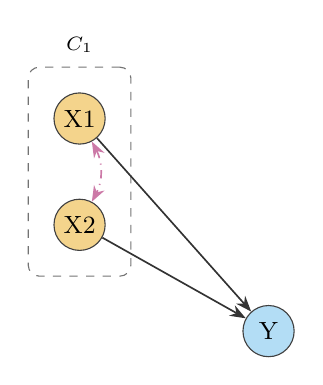
\begin{tikzpicture}
  \node[mannode] (nX1) at (0.00,0.00) {X1};
  \node[mannode] (nX2) at (0.00,-1.35) {X2};
  \node[tgtnode] (nY) at (2.40,-2.70) {Y};
  \draw[diredge] (nX1) -- (nY);
  \draw[diredge] (nX2) -- (nY);
  \draw[biintra] (nX1) to[bend left=28] (nX2);
  \begin{scope}[on background layer]
    \node[clbox,fit=(nX1)(nX2),label={[label distance=0.5mm]above:{\scriptsize$C_{1}$}}] {};
  \end{scope}
\end{tikzpicture}}\hfill
\adjustbox{max width=0.38\linewidth,valign=c}{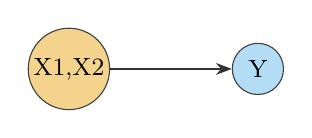
\begin{tikzpicture}
  \node[tgtnode] (nY) at (2.40,0.00) {Y};
  \node[mannode] (nX1X2) at (0.00,0.00) {X1,X2};
  \draw[diredge] (nX1X2) -- (nY);
\end{tikzpicture}}
\caption{\textbf{ParallelParent (MinimalBench, Exp.\ A).} Fine DAG with coarse partition (left) and quotient C-DAG (right), in the convention of Fig.~\ref{fig:motivating}: manipulable variables orange, target blue, dash-dotted latent confounding; dashed boxes are the manipulable clusters. The intra-cluster $X_1\leftrightarrow X_2$ disappears in the quotient; deleting $X_1\to Y$ leaves $C_1\to Y$ alive through $X_2\to Y$ (quotient-redundant).}
\label{fig:dag-parallelparent}
\end{figure}

\begin{figure}[t]\centering
\adjustbox{max width=0.58\linewidth,valign=c}{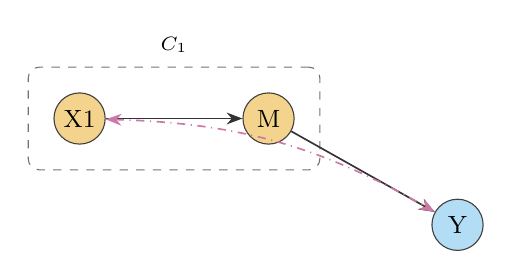
\begin{tikzpicture}
  \node[mannode] (nX1) at (0.00,0.00) {X1};
  \node[mannode] (nM) at (2.40,0.00) {M};
  \node[tgtnode] (nY) at (4.80,-1.35) {Y};
  \draw[diredge] (nX1) -- (nM);
  \draw[diredge] (nM) -- (nY);
  \draw[bicross] (nX1) to[bend left=14] (nY);
  \begin{scope}[on background layer]
    \node[clbox,fit=(nX1)(nM),label={[label distance=0.5mm]above:{\scriptsize$C_{1}$}}] {};
  \end{scope}
\end{tikzpicture}}\hfill
\adjustbox{max width=0.38\linewidth,valign=c}{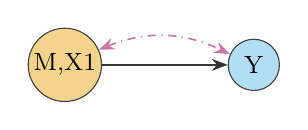
\begin{tikzpicture}
  \node[mannode] (nMX1) at (0.00,0.00) {M,X1};
  \node[tgtnode] (nY) at (2.40,0.00) {Y};
  \draw[diredge] (nMX1) -- (nY);
  \draw[bicross] (nMX1) to[bend left=24] (nY);
\end{tikzpicture}}
\caption{\textbf{FrontDoor (MinimalBench, Exp.\ B).} Fine DAG with coarse partition (left) and quotient C-DAG (right), in the convention of Fig.~\ref{fig:motivating}: manipulable variables orange, target blue, dash-dotted latent confounding; dashed boxes are the manipulable clusters. The quotient is a bow ($C_1\to Y$, $C_1\leftrightarrow Y$): the cluster arm runs on the uninformative prior tier in every condition, so the assumed intra-cluster $X_1\leftrightarrow M$ cannot change it.}
\label{fig:dag-frontdoor}
\end{figure}

\begin{figure}[t]\centering
\adjustbox{max width=0.58\linewidth,valign=c}{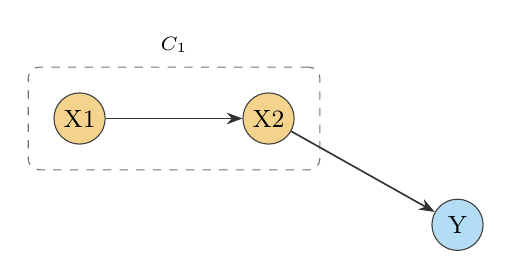
\begin{tikzpicture}
  \node[mannode] (nX1) at (0.00,0.00) {X1};
  \node[mannode] (nX2) at (2.40,0.00) {X2};
  \node[tgtnode] (nY) at (4.80,-1.35) {Y};
  \draw[diredge] (nX1) -- (nX2);
  \draw[diredge] (nX2) -- (nY);
  \begin{scope}[on background layer]
    \node[clbox,fit=(nX1)(nX2),label={[label distance=0.5mm]above:{\scriptsize$C_{1}$}}] {};
  \end{scope}
\end{tikzpicture}}\hfill
\adjustbox{max width=0.38\linewidth,valign=c}{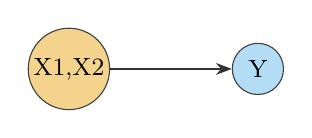
\begin{tikzpicture}
  \node[tgtnode] (nY) at (2.40,0.00) {Y};
  \node[mannode] (nX1X2) at (0.00,0.00) {X1,X2};
  \draw[diredge] (nX1X2) -- (nY);
\end{tikzpicture}}
\caption{\textbf{MediatedChain (MinimalBench, Exp.\ C).} Fine DAG with coarse partition (left) and quotient C-DAG (right), in the convention of Fig.~\ref{fig:motivating}: manipulable variables orange, target blue, dash-dotted latent confounding; dashed boxes are the manipulable clusters. The policy box restricts $D(X_2)$ to $[-2,2]$; the fine optimum $\doo(X_1{=}2)$ drives $X_2$ to $4$, outside the box.}
\label{fig:dag-mediatedchain}
\end{figure}

\begin{figure}[t]\centering
\adjustbox{max width=0.58\linewidth,valign=c}{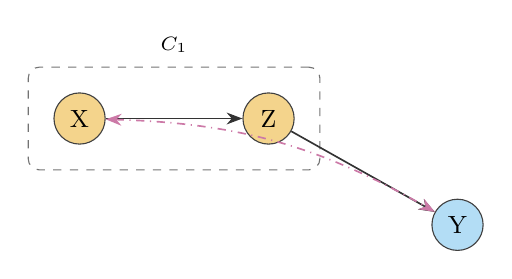
\begin{tikzpicture}
  \node[mannode] (nX) at (0.00,0.00) {X};
  \node[mannode] (nZ) at (2.40,0.00) {Z};
  \node[tgtnode] (nY) at (4.80,-1.35) {Y};
  \draw[diredge] (nX) -- (nZ);
  \draw[diredge] (nZ) -- (nY);
  \draw[bicross] (nX) to[bend left=14] (nY);
  \begin{scope}[on background layer]
    \node[clbox,fit=(nX)(nZ),label={[label distance=0.5mm]above:{\scriptsize$C_{1}$}}] {};
  \end{scope}
\end{tikzpicture}}\hfill
\adjustbox{max width=0.38\linewidth,valign=c}{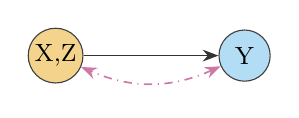
\begin{tikzpicture}
  \node[tgtnode] (nY) at (2.40,0.00) {Y};
  \node[mannode] (nXZ) at (0.00,0.00) {X,Z};
  \draw[diredge] (nXZ) -- (nY);
  \draw[bicross] (nY) to[bend left=24] (nXZ);
\end{tikzpicture}}
\caption{\textbf{ToyGraph (CBO family).} Fine DAG with coarse partition (left) and quotient C-DAG (right), in the convention of Fig.~\ref{fig:motivating}: manipulable variables orange, target blue, dash-dotted latent confounding; dashed boxes are the manipulable clusters. The quotient is a bow ($C_1\to Y$, $C_1\leftrightarrow Y$): $\doo(C_1)$ is not identifiable from the C-DAG, so the arm runs on the uninformative prior tier.}
\label{fig:dag-toy}
\end{figure}

\begin{figure}[t]\centering
\adjustbox{max width=0.58\linewidth,valign=c}{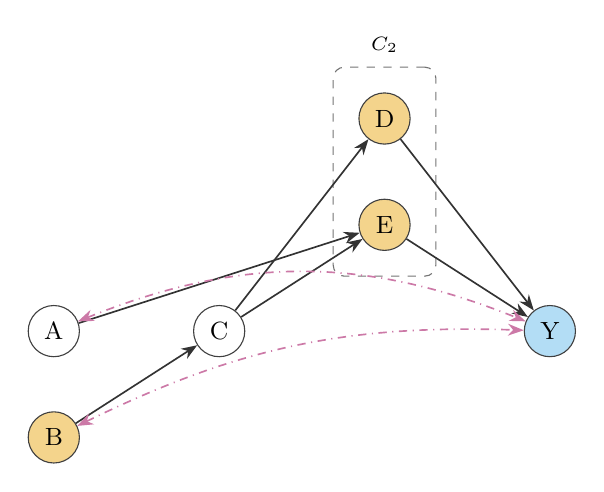
\begin{tikzpicture}
  \node[obsnode] (nA) at (0.00,-2.70) {A};
  \node[mannode] (nB) at (0.00,-4.05) {B};
  \node[obsnode] (nC) at (2.10,-2.70) {C};
  \node[mannode] (nD) at (4.20,0.00) {D};
  \node[mannode] (nE) at (4.20,-1.35) {E};
  \node[tgtnode] (nY) at (6.30,-2.70) {Y};
  \draw[diredge] (nB) -- (nC);
  \draw[diredge] (nC) -- (nD);
  \draw[diredge] (nA) -- (nE);
  \draw[diredge] (nC) -- (nE);
  \draw[diredge] (nD) -- (nY);
  \draw[diredge] (nE) -- (nY);
  \draw[bicross] (nB) to[bend left=14] (nY);
  \draw[bicross] (nA) to[bend left=22] (nY);
  \begin{scope}[on background layer]
    \node[clbox,fit=(nD)(nE),label={[label distance=0.5mm]above:{\scriptsize$C_{2}$}}] {};
  \end{scope}
\end{tikzpicture}}\hfill
\adjustbox{max width=0.38\linewidth,valign=c}{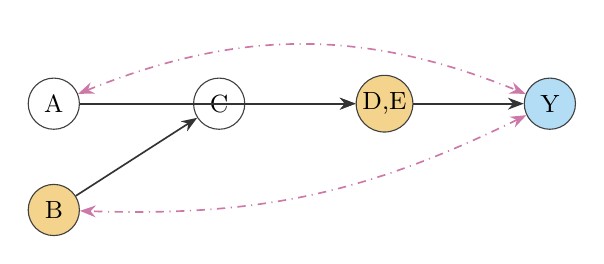
\begin{tikzpicture}
  \node[mannode] (nB) at (0.00,-1.35) {B};
  \node[obsnode] (nC) at (2.10,0.00) {C};
  \node[obsnode] (nA) at (0.00,0.00) {A};
  \node[mannode] (nDE) at (4.20,0.00) {D,E};
  \node[tgtnode] (nY) at (6.30,0.00) {Y};
  \draw[diredge] (nC) -- (nDE);
  \draw[diredge] (nB) -- (nC);
  \draw[diredge] (nA) -- (nDE);
  \draw[diredge] (nDE) -- (nY);
  \draw[bicross] (nY) to[bend left=14] (nB);
  \draw[bicross] (nA) to[bend left=22] (nY);
\end{tikzpicture}}
\caption{\textbf{CompleteGraph (CBO family).} Fine DAG with coarse partition (left) and quotient C-DAG (right), in the convention of Fig.~\ref{fig:motivating}: manipulable variables orange, target blue, dash-dotted latent confounding; dashed boxes are the manipulable clusters.}
\label{fig:dag-complete}
\end{figure}

\begin{figure}[t]\centering
\adjustbox{max width=0.58\linewidth,valign=c}{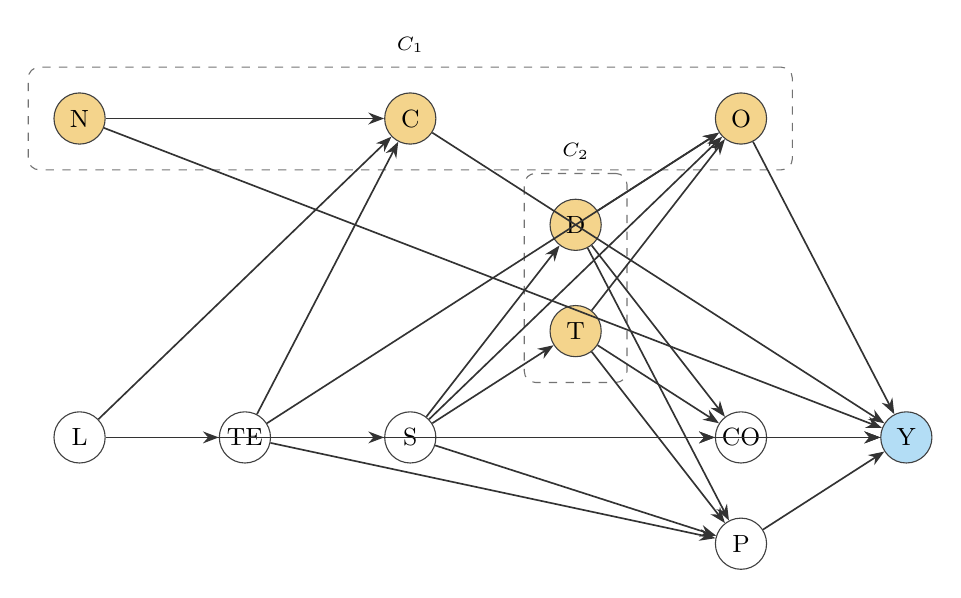
\begin{tikzpicture}
  \node[mannode] (nN) at (0.00,0.00) {N};
  \node[obsnode] (nL) at (0.00,-4.05) {L};
  \node[obsnode] (nTE) at (2.10,-4.05) {TE};
  \node[mannode] (nC) at (4.20,0.00) {C};
  \node[obsnode] (nS) at (4.20,-4.05) {S};
  \node[mannode] (nT) at (6.30,-2.70) {T};
  \node[mannode] (nD) at (6.30,-1.35) {D};
  \node[obsnode] (nP) at (8.40,-5.40) {P};
  \node[mannode] (nO) at (8.40,0.00) {O};
  \node[obsnode] (nCO) at (8.40,-4.05) {CO};
  \node[tgtnode] (nY) at (10.50,-4.05) {Y};
  \draw[diredge] (nL) -- (nTE);
  \draw[diredge] (nL) -- (nC);
  \draw[diredge] (nL) -- (nY);
  \draw[diredge] (nN) -- (nC);
  \draw[diredge] (nN) -- (nY);
  \draw[diredge] (nTE) -- (nC);
  \draw[diredge] (nTE) -- (nS);
  \draw[diredge] (nTE) -- (nP);
  \draw[diredge] (nTE) -- (nO);
  \draw[diredge] (nTE) -- (nCO);
  \draw[diredge] (nTE) -- (nY);
  \draw[diredge] (nS) -- (nT);
  \draw[diredge] (nS) -- (nD);
  \draw[diredge] (nS) -- (nP);
  \draw[diredge] (nS) -- (nO);
  \draw[diredge] (nS) -- (nCO);
  \draw[diredge] (nT) -- (nP);
  \draw[diredge] (nT) -- (nO);
  \draw[diredge] (nT) -- (nCO);
  \draw[diredge] (nD) -- (nP);
  \draw[diredge] (nD) -- (nO);
  \draw[diredge] (nD) -- (nCO);
  \draw[diredge] (nP) -- (nY);
  \draw[diredge] (nO) -- (nY);
  \draw[diredge] (nC) -- (nY);
  \draw[diredge] (nCO) -- (nY);
  \begin{scope}[on background layer]
    \node[clbox,fit=(nC)(nN)(nO),label={[label distance=0.5mm]above:{\scriptsize$C_{1}$}}] {};
  \end{scope}
  \begin{scope}[on background layer]
    \node[clbox,fit=(nD)(nT),label={[label distance=0.5mm]above:{\scriptsize$C_{2}$}}] {};
  \end{scope}
\end{tikzpicture}}\hfill
\adjustbox{max width=0.38\linewidth,valign=c}{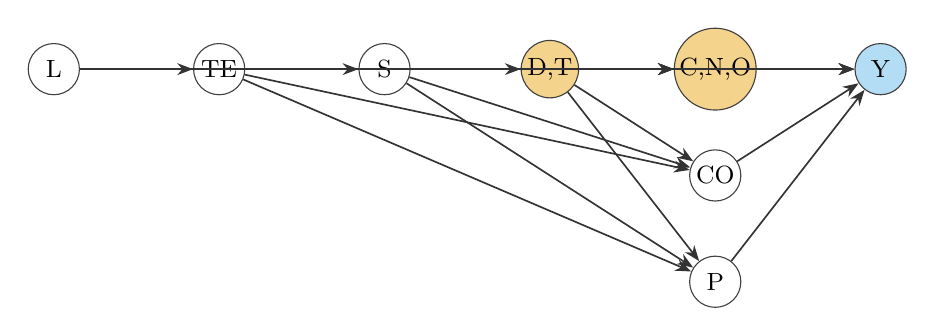
\begin{tikzpicture}
  \node[mannode] (nDT) at (6.30,0.00) {D,T};
  \node[obsnode] (nTE) at (2.10,0.00) {TE};
  \node[mannode] (nCNO) at (8.40,0.00) {C,N,O};
  \node[obsnode] (nS) at (4.20,0.00) {S};
  \node[obsnode] (nCO) at (8.40,-1.35) {CO};
  \node[obsnode] (nP) at (8.40,-2.70) {P};
  \node[obsnode] (nL) at (0.00,0.00) {L};
  \node[tgtnode] (nY) at (10.50,0.00) {Y};
  \draw[diredge] (nL) -- (nY);
  \draw[diredge] (nS) -- (nCNO);
  \draw[diredge] (nCNO) -- (nY);
  \draw[diredge] (nTE) -- (nCNO);
  \draw[diredge] (nTE) -- (nP);
  \draw[diredge] (nDT) -- (nCNO);
  \draw[diredge] (nS) -- (nCO);
  \draw[diredge] (nL) -- (nTE);
  \draw[diredge] (nP) -- (nY);
  \draw[diredge] (nDT) -- (nCO);
  \draw[diredge] (nTE) -- (nCO);
  \draw[diredge] (nDT) -- (nP);
  \draw[diredge] (nL) -- (nCNO);
  \draw[diredge] (nS) -- (nP);
  \draw[diredge] (nCO) -- (nY);
  \draw[diredge] (nS) -- (nDT);
  \draw[diredge] (nTE) -- (nY);
  \draw[diredge] (nTE) -- (nS);
\end{tikzpicture}}
\caption{\textbf{SimplifiedCoralGraph (CBO family).} Fine DAG with coarse partition (left) and quotient C-DAG (right), in the convention of Fig.~\ref{fig:motivating}: manipulable variables orange, target blue, dash-dotted latent confounding; dashed boxes are the manipulable clusters.}
\label{fig:dag-coral}
\end{figure}

\begin{figure}[t]\centering
\adjustbox{max width=0.58\linewidth,valign=c}{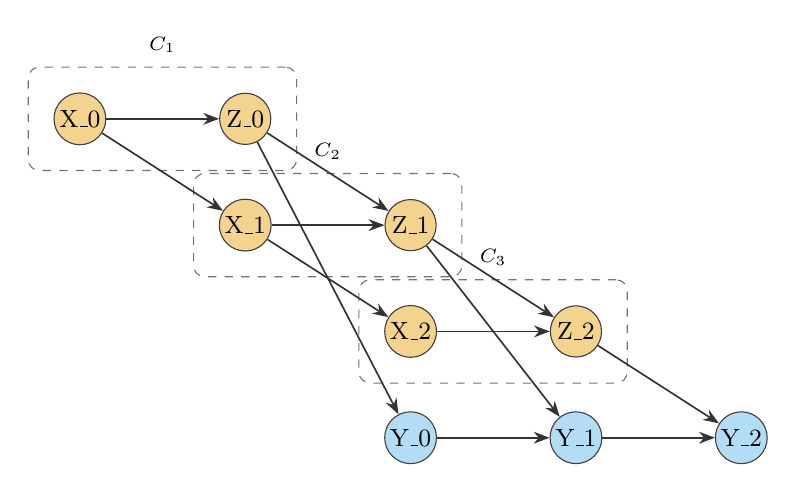
\begin{tikzpicture}
  \node[mannode] (nX0) at (0.00,0.00) {X\_0};
  \node[mannode] (nZ0) at (2.10,0.00) {Z\_0};
  \node[tgtnode] (nY0) at (4.20,-4.05) {Y\_0};
  \node[mannode] (nX1) at (2.10,-1.35) {X\_1};
  \node[mannode] (nZ1) at (4.20,-1.35) {Z\_1};
  \node[tgtnode] (nY1) at (6.30,-4.05) {Y\_1};
  \node[mannode] (nX2) at (4.20,-2.70) {X\_2};
  \node[mannode] (nZ2) at (6.30,-2.70) {Z\_2};
  \node[tgtnode] (nY2) at (8.40,-4.05) {Y\_2};
  \draw[diredge] (nX0) -- (nZ0);
  \draw[diredge] (nZ0) -- (nY0);
  \draw[diredge] (nX1) -- (nZ1);
  \draw[diredge] (nZ1) -- (nY1);
  \draw[diredge] (nX2) -- (nZ2);
  \draw[diredge] (nZ2) -- (nY2);
  \draw[diredge] (nX0) -- (nX1);
  \draw[diredge] (nZ0) -- (nZ1);
  \draw[diredge] (nY0) -- (nY1);
  \draw[diredge] (nX1) -- (nX2);
  \draw[diredge] (nZ1) -- (nZ2);
  \draw[diredge] (nY1) -- (nY2);
  \begin{scope}[on background layer]
    \node[clbox,fit=(nX0)(nZ0),label={[label distance=0.5mm]above:{\scriptsize$C_{1}$}}] {};
  \end{scope}
  \begin{scope}[on background layer]
    \node[clbox,fit=(nX1)(nZ1),label={[label distance=0.5mm]above:{\scriptsize$C_{2}$}}] {};
  \end{scope}
  \begin{scope}[on background layer]
    \node[clbox,fit=(nX2)(nZ2),label={[label distance=0.5mm]above:{\scriptsize$C_{3}$}}] {};
  \end{scope}
\end{tikzpicture}}\hfill
\adjustbox{max width=0.38\linewidth,valign=c}{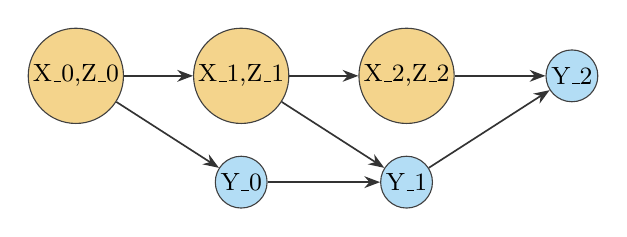
\begin{tikzpicture}
  \node[mannode] (nX0Z0) at (0.00,0.00) {X\_0,Z\_0};
  \node[tgtnode] (nY0) at (2.10,-1.35) {Y\_0};
  \node[mannode] (nX1Z1) at (2.10,0.00) {X\_1,Z\_1};
  \node[tgtnode] (nY1) at (4.20,-1.35) {Y\_1};
  \node[mannode] (nX2Z2) at (4.20,0.00) {X\_2,Z\_2};
  \node[tgtnode] (nY2) at (6.30,0.00) {Y\_2};
  \draw[diredge] (nX0Z0) -- (nY0);
  \draw[diredge] (nX1Z1) -- (nY1);
  \draw[diredge] (nX2Z2) -- (nY2);
  \draw[diredge] (nX0Z0) -- (nX1Z1);
  \draw[diredge] (nY0) -- (nY1);
  \draw[diredge] (nX1Z1) -- (nX2Z2);
  \draw[diredge] (nY1) -- (nY2);
\end{tikzpicture}}
\caption{\textbf{DCBO stat / nonstat (QDCBO family).} Fine DAG with coarse partition (left) and quotient C-DAG (right), in the convention of Fig.~\ref{fig:motivating}: manipulable variables orange, target blue, dash-dotted latent confounding; dashed boxes are the manipulable clusters. Slices $t=0,1,2$; the nonstat setup shares this topology with a change point in the SEM.}
\label{fig:dag-dcbo-stat}
\end{figure}

\begin{figure}[t]\centering
\adjustbox{max width=0.58\linewidth,valign=c}{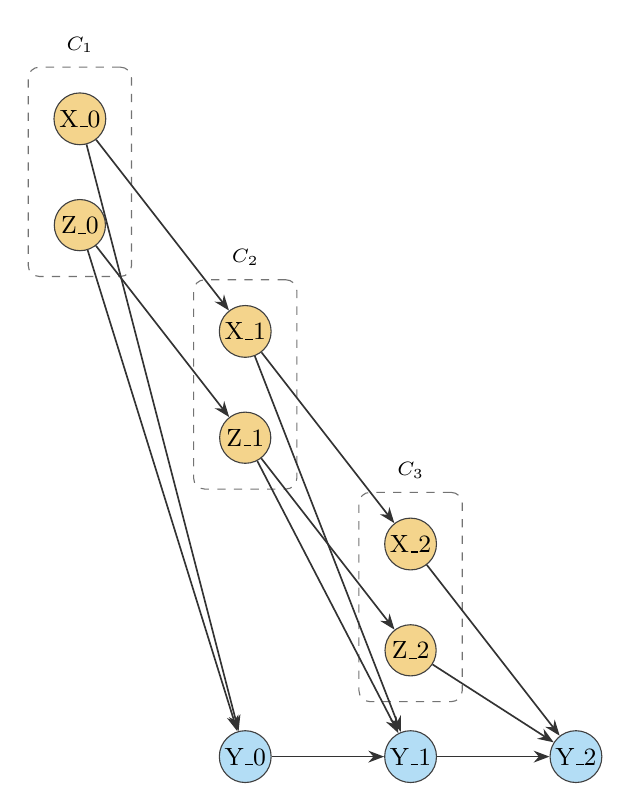
\begin{tikzpicture}
  \node[mannode] (nX0) at (0.00,0.00) {X\_0};
  \node[mannode] (nZ0) at (0.00,-1.35) {Z\_0};
  \node[tgtnode] (nY0) at (2.10,-8.10) {Y\_0};
  \node[mannode] (nX1) at (2.10,-2.70) {X\_1};
  \node[mannode] (nZ1) at (2.10,-4.05) {Z\_1};
  \node[tgtnode] (nY1) at (4.20,-8.10) {Y\_1};
  \node[mannode] (nX2) at (4.20,-5.40) {X\_2};
  \node[mannode] (nZ2) at (4.20,-6.75) {Z\_2};
  \node[tgtnode] (nY2) at (6.30,-8.10) {Y\_2};
  \draw[diredge] (nX0) -- (nY0);
  \draw[diredge] (nZ0) -- (nY0);
  \draw[diredge] (nX1) -- (nY1);
  \draw[diredge] (nZ1) -- (nY1);
  \draw[diredge] (nX2) -- (nY2);
  \draw[diredge] (nZ2) -- (nY2);
  \draw[diredge] (nX0) -- (nX1);
  \draw[diredge] (nZ0) -- (nZ1);
  \draw[diredge] (nY0) -- (nY1);
  \draw[diredge] (nX1) -- (nX2);
  \draw[diredge] (nZ1) -- (nZ2);
  \draw[diredge] (nY1) -- (nY2);
  \begin{scope}[on background layer]
    \node[clbox,fit=(nX0)(nZ0),label={[label distance=0.5mm]above:{\scriptsize$C_{1}$}}] {};
  \end{scope}
  \begin{scope}[on background layer]
    \node[clbox,fit=(nX1)(nZ1),label={[label distance=0.5mm]above:{\scriptsize$C_{2}$}}] {};
  \end{scope}
  \begin{scope}[on background layer]
    \node[clbox,fit=(nX2)(nZ2),label={[label distance=0.5mm]above:{\scriptsize$C_{3}$}}] {};
  \end{scope}
\end{tikzpicture}}\hfill
\adjustbox{max width=0.38\linewidth,valign=c}{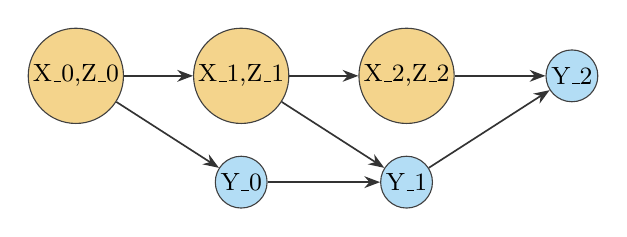
\begin{tikzpicture}
  \node[mannode] (nX0Z0) at (0.00,0.00) {X\_0,Z\_0};
  \node[tgtnode] (nY0) at (2.10,-1.35) {Y\_0};
  \node[mannode] (nX1Z1) at (2.10,0.00) {X\_1,Z\_1};
  \node[tgtnode] (nY1) at (4.20,-1.35) {Y\_1};
  \node[mannode] (nX2Z2) at (4.20,0.00) {X\_2,Z\_2};
  \node[tgtnode] (nY2) at (6.30,0.00) {Y\_2};
  \draw[diredge] (nX0Z0) -- (nY0);
  \draw[diredge] (nX1Z1) -- (nY1);
  \draw[diredge] (nX2Z2) -- (nY2);
  \draw[diredge] (nX0Z0) -- (nX1Z1);
  \draw[diredge] (nY0) -- (nY1);
  \draw[diredge] (nX1Z1) -- (nX2Z2);
  \draw[diredge] (nY1) -- (nY2);
\end{tikzpicture}}
\caption{\textbf{DCBO ind (QDCBO family).} Fine DAG with coarse partition (left) and quotient C-DAG (right), in the convention of Fig.~\ref{fig:motivating}: manipulable variables orange, target blue, dash-dotted latent confounding; dashed boxes are the manipulable clusters.}
\label{fig:dag-dcbo-ind}
\end{figure}

\begin{figure}[t]\centering
\adjustbox{max width=0.58\linewidth,valign=c}{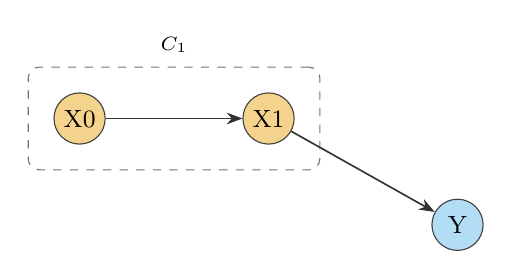
\begin{tikzpicture}
  \node[mannode] (nX0) at (0.00,0.00) {X0};
  \node[mannode] (nX1) at (2.40,0.00) {X1};
  \node[tgtnode] (nY) at (4.80,-1.35) {Y};
  \draw[diredge] (nX0) -- (nX1);
  \draw[diredge] (nX1) -- (nY);
  \begin{scope}[on background layer]
    \node[clbox,fit=(nX0)(nX1),label={[label distance=0.5mm]above:{\scriptsize$C_{1}$}}] {};
  \end{scope}
\end{tikzpicture}}\hfill
\adjustbox{max width=0.38\linewidth,valign=c}{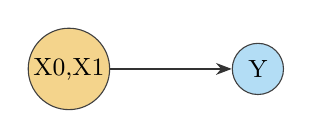
\begin{tikzpicture}
  \node[mannode] (nX0X1) at (0.00,0.00) {X0,X1};
  \node[tgtnode] (nY) at (2.40,0.00) {Y};
  \draw[diredge] (nX0X1) -- (nY);
\end{tikzpicture}}
\caption{\textbf{ToyGraph-M (QMCBO family).} Fine DAG with coarse partition (left) and quotient C-DAG (right), in the convention of Fig.~\ref{fig:motivating}: manipulable variables orange, target blue, dash-dotted latent confounding; dashed boxes are the manipulable clusters.}
\label{fig:dag-mcbo-toygraph-m}
\end{figure}

\begin{figure}[t]\centering
\adjustbox{max width=0.58\linewidth,valign=c}{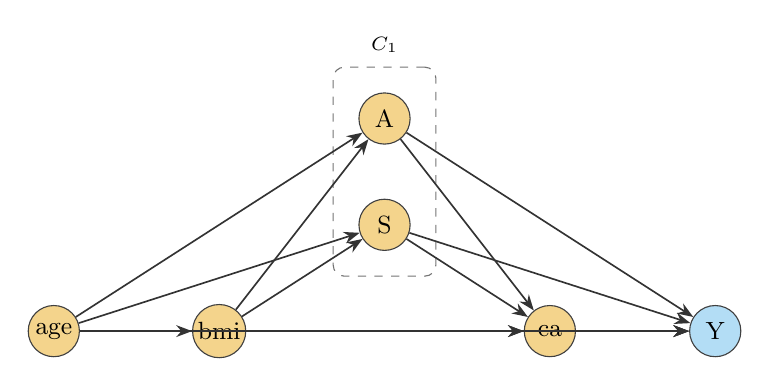
\begin{tikzpicture}
  \node[mannode] (nage) at (0.00,-2.70) {age};
  \node[mannode] (nbmi) at (2.10,-2.70) {bmi};
  \node[mannode] (nA) at (4.20,0.00) {A};
  \node[mannode] (nS) at (4.20,-1.35) {S};
  \node[mannode] (nca) at (6.30,-2.70) {ca};
  \node[tgtnode] (nY) at (8.40,-2.70) {Y};
  \draw[diredge] (nage) -- (nbmi);
  \draw[diredge] (nage) -- (nA);
  \draw[diredge] (nbmi) -- (nA);
  \draw[diredge] (nage) -- (nS);
  \draw[diredge] (nbmi) -- (nS);
  \draw[diredge] (nage) -- (nca);
  \draw[diredge] (nbmi) -- (nca);
  \draw[diredge] (nA) -- (nca);
  \draw[diredge] (nS) -- (nca);
  \draw[diredge] (nage) -- (nY);
  \draw[diredge] (nbmi) -- (nY);
  \draw[diredge] (nA) -- (nY);
  \draw[diredge] (nS) -- (nY);
  \draw[diredge] (nca) -- (nY);
  \begin{scope}[on background layer]
    \node[clbox,fit=(nA)(nS),label={[label distance=0.5mm]above:{\scriptsize$C_{1}$}}] {};
  \end{scope}
\end{tikzpicture}}\hfill
\adjustbox{max width=0.38\linewidth,valign=c}{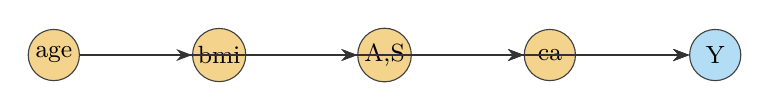
\begin{tikzpicture}
  \node[mannode] (nage) at (0.00,0.00) {age};
  \node[mannode] (nbmi) at (2.10,0.00) {bmi};
  \node[mannode] (nAS) at (4.20,0.00) {A,S};
  \node[mannode] (nca) at (6.30,0.00) {ca};
  \node[tgtnode] (nY) at (8.40,0.00) {Y};
  \draw[diredge] (nage) -- (nbmi);
  \draw[diredge] (nage) -- (nAS);
  \draw[diredge] (nbmi) -- (nAS);
  \draw[diredge] (nage) -- (nca);
  \draw[diredge] (nbmi) -- (nca);
  \draw[diredge] (nAS) -- (nca);
  \draw[diredge] (nage) -- (nY);
  \draw[diredge] (nbmi) -- (nY);
  \draw[diredge] (nAS) -- (nY);
  \draw[diredge] (nca) -- (nY);
\end{tikzpicture}}
\caption{\textbf{PSAGraph (QMCBO family).} Fine DAG with coarse partition (left) and quotient C-DAG (right), in the convention of Fig.~\ref{fig:motivating}: manipulable variables orange, target blue, dash-dotted latent confounding; dashed boxes are the manipulable clusters.}
\label{fig:dag-mcbo-psagraph}
\end{figure}


\endgroup
\clearpage

\end{document}
